\documentclass[a4paper,12pt]{report}

\usepackage[english]{babel}
\usepackage[utf8]{inputenc}
\usepackage[T1]{fontenc}
\usepackage{amsmath}
\usepackage{graphicx}
\usepackage{titlesec}
\usepackage{wrapfig}
\usepackage{float}
\usepackage{calc}
\usepackage{url}
\def\UrlBreaks{\do\/\do-}
\usepackage{enumitem}
\usepackage{etoolbox}
\usepackage{tabularx}
\usepackage{placeins}
\usepackage{setspace}
\usepackage{booktabs}
\usepackage{tcolorbox}
\usepackage[
  inner=3cm,       
  outer=2.5cm,     
  top=2.5cm,
  bottom=2.5cm,
  bindingoffset=5mm,% extra Einzug für Bindung, wenn benötigt
]{geometry}
\usepackage[backend=biber,style=numeric,sorting=none]{biblatex}
\addbibresource{references.bib}



\setlength{\parindent}{0pt}

\titleformat{\chapter}[hang]
  {\normalfont\huge\bfseries}
  {\thechapter\quad} % This is the number (e.g. "1")
  {0pt}
  {} % No label text like "Chapter"



\begin{document}





\thispagestyle{empty}

% Fakultät (oben, mitte)
\begin{center}
  \large
University of Leipzig\\
Faculty of Mathematics and Computer Science\\[0.3cm]
Institute of Computer Science
\end{center}

\vspace{3cm}

% Title (Mitte, mitte)
\begin{center}
  \LARGE\bfseries
  Bachelor's Thesis\\[1cm]
  Comparative Study about predictive performance of Machine Learning algorithms\\
  in forecasting stock prices of different volatility
\end{center}

\vspace{3cm}

% Author (unter Titel mitte)
\begin{center}
  \large
  Jeremias Lukas Aechtner
\end{center}

\vfill

% Bottom left and right lines
\noindent
\begin{minipage}[t]{0.5\textwidth}
  Leipzig, 07.2025
\end{minipage}%
\begin{minipage}[t]{0.5\textwidth}
  \raggedleft
  submitted by Jeremias Lukas Aechtner,\\
  Course of study: Informatik B. SC.
\end{minipage}

\vspace{2cm}

% Supervisors (ganz unten links)
\noindent
\begin{minipage}[t]{\textwidth}
  \small
  \textbf{Supervising university lecturer:}\\
  Prof. Gregory Provan, School of Computer Science and Information Technology, University College Cork\\
  Prof. Dr. Andreas Maletti, Fakultät für Mathematik und Informatik, Universität Leipzig
\end{minipage}


\newpage
\vspace*{\fill}

{\fontsize{20}{23}\selectfont\textbf{Abstract}}\\\\\\\\




In the financial world various machine learning techniques are applied to different tasks. They are used to manage risk and predict price movements for every kind of asset. Forecasting accuracy as well as efficiency thereby play a major role. Therefore in this thesis we wanted to evaluate the performance of three machine learning models that were trained on stocks and ETFs with different volatility. This thesis compares their performance and investigates what impact the volatility of the training data has. The models we used are LSTM, CNN and XGBoost. A variety of technical and macro-economic indicators was added as features. The XGBoost model performed outstandingly. With approximately one hour execution time it was 32 times faster than the LSTM and about 4.5 times faster than the CNN model while having the best overall error. The LSTM is close behind the XGBoost in terms of predictive accuracy and the CNN has a much higher error. The thesis was aimed to show relations of predictive accuracy and certain characteristics in the data while focusing on the volatility as a characteristic. This can help to clarify strengths and weaknesses of certain models when applied to more or less volatile assets. Some further research questions are suggested in the end.
\vspace{6cm}
\vspace*{\fill}












\newpage
\begin{center}
\begin{minipage}{\textwidth}
\vspace{2cm}
\section*{Acknowledgment}

\vspace{1cm}


I would like to thank Professor Gregory Provan from the School of Computer Science and Information Technology at the University College Cork and Professor Andreas Maletti, PhD from the faculty for mathematics and computer science at the University Leipzig who agreed to supervise me on this topic. I always received their guidance and honest opinion as an invaluable support for both the development of the content of the thesis and the general process. I would like to thank the School of Computer Science and Information Technology from the University College Cork and the Faculty for Mathematics and Computer Science from the University Leipzig who have been very supportive with all formal matters. Furthermore I would like to thank the international office at the UCC and the Office of International Affairs at the University Leipzig that made it possible for me to write this thesis in the context of my Erasmus exchange stay in Ireland. I would like to express my sincere gratitude towards my friends and family that supported me in many different ways throughout the entire process. \\
\\
\\


\end{minipage}
\end{center}

\newpage

\chapter*{Glossary}

\begin{description}
  \item[Self‑updating system] A system that automatically adjusts its internal parameters based on incoming data (i.e.\ it “learns”).

  \item[Prediction error] The difference between the system’s predicted value and the true value.

  \item[Learning] The process by which a system updates its parameters in response to the prediction error in order to improve over time.

  \item[Data point] A single observation in the dataset, represented by a feature vector (one row in a table).

  \item[Period] A time interval corresponding to one measurement instance. (e.g.\ Day, minute, hour).

  \item[Feature] An individual measurable property or characteristic of a data point.

  \item[Data set] A collection of data points, typically organized as a table whose rows are periods and whose columns are features.

  \item[Adding a feature] Introducing a new variable to the dataset—i.e.\ appending a column so that each data point can gain that attribute.

  \item[Classification] A supervised learning task where the target output is categorical (e.g.\ “spam” vs.\ “not spam”).

  \item[Regression] A supervised learning task where the target output is a continuous value (e.g.\ predicting a house price).

  \item[Overfitting] When a model learns characteristics of only the training data too well, capturing noise or random fluctuations, resulting in poor performance on new, unseen data.

  \item[Generalization] The ability of a trained model to make accurate predictions on new, unseen data — not just on its training set.
\end{description}



\tableofcontents
\listoffigures
\newpage





\chapter{Introduction}
Machine learning has become a very important technology. It is applied to many tasks which can be split into different subareas. One of those areas is time series forecasting where people try to predict a future sequence or element based on a past sequence or element. There it is applied it to a variety of real-world challenges. These fields include Healthcare \cite{1}, Energy \cite{2}, Agriculture \cite{3}, Climate \& Weather \cite{4} and financial data. Machine Learning is a currently rapidly evolving technology for which people find new use cases permanently. The ways it can be applied to problems and challenges are various and numerous. Besides predicting customer behavior in stores, predicting energy consumption over time or analyzing biometric data to conclude about health status, it is also widely applied to predict economic parameters. Business consultancy companies make big use of these algorithms to facilitate and improve the quality of their service. A similar sector in which this technology is applied regularly is finance. Machine learning is used to flag in real time anomalies in transactions to detect fraud or money laundry which allows for immediate intervention \cite{58}. It is used to calculate credit scores and manage risk of credits based on a wider range of borrower data than traditional credit-bureau scores \cite{59}. Besides that, it is widely used in trading to asses the quality of an asset, the risk of an investment, the potential upside of a stock or simply to give recommendations on buy or sell orders for traders. Many big trading companies apply algorithms that execute orders automatically given certain circumstances. There is a lot of potential profit in this area which is why many parties are chasing the idea of creating a trading algorithm that can outperform the market. The efficient market hypothesis contradicts this vision. It is a hypothesis after which at any given moment the prices of assets fully reflect all possibly available information about that asset \cite{60}. After that it would be impossible to outperform the market since the price only changes with information which was impossible to foresee. There are three forms of this hypothesis. The weak form states that prices reflect all past market data. Based on that it would be impossible to outperform the market by only using past market data. The semi-strong form says that prices reflect all publicly available information. Following that means it would be only possible to outperform the market if you had insider information. And finally, there is the strong form. Considering the strong form, prices reflect all information including public and insider information which makes it overall impossible to outperform the market. Often the prices change when new unexpected information become publicly available. This is why time and speed matter a lot in these trading firms and it is the reason they optimize their infrastructure and reaction speed as much as possible. There are certain traders and companies who in fact do consistently outperform the market. That leads to the assumption that the hypothesis’ strong form isn’t the one representing the stock market dynamics of our world. A currently realistic form would probably be located somewhere between the semi-strong and strong form but we don’t know it exactly. Because of that, people still are looking for ways to outperform the market which leads to this huge research area of stock and asset price forecasting. There are many different ways to employ machine learning in this area. From forecasting concrete stock prices over analyzing the risk of one asset to only giving binary recommendations whether one should sell short or buy long of an ETF. Stock price forecasting is one of those many fields that are heavily developing. Many findings have already been made in this area in applying machine learning algorithms. \\
\\
We will briefly discover the current state of the art throughout the following literature review and following that we want to contribute with this thesis to this research area.



\chapter{Literature Review}
The paper \cite{5} from Kumbure et al. (2022) showed in a comprehensive review the technological development in the field of stock forecasting. The review includes 138 articles that have been published between 2000 and 2019. It looks on machine learning techniques that have been applied, features that were considered for training and metrics with which results have been measured. Like that they propose a differentiation of features into 4 categories which are “Technical Indicators”, “Macro-Economy”, “Fundamental Indicators” and “others”. They explain the importance of these features and how often they are used. In section 5.4.8 that review \cite{5} illustrates what families of machine learning models have been applied to the task of forecasting stock prices. It shows that at least since the year 2000 Artificial Neural Networks (ANNs) in various forms were experimented with heavily. \\
\\\
One representative of Artificial Neural Networks is mentioned very regularly in research – Long Short-Term Memory (LSTM). The paper \cite{6} by Matharasi et al. (2025) evaluates two models against each other which are LSTM and XGBoost. Both delivered promising accuracy in forecasting AMD inc. stock data. While the LSTM model delivered slightly better accuracy in forecasts, the XGBoost model could excel in computational efficiency. Both models have been shown to have outstanding in predictive performance when forecasting certain stock or index data. Teixeira, D. M., \& Barbosa, R. S. (2025) have conducted another experiment \cite{13} that shows their effectiveness in capturing the complexity of stock prices. They evaluate the models LSTM and XGBoost as well as other architectures such as GRU, CNN, RNN, but also different hybrid combinations of these like LSTM + CNN, RNN + GRU, GRU + CNN, LSTM + GRU, and RNN + LSTM. The study trains all of these models on historical stock data from Apple inc. and comes to the result that the standalone models of GRU, LSTM and XGBoost perform the best for the Apple inc. stock data. This is a little counterintuitive since one might think that hybrid models usually outperform their standalone component models since they might merge strengths of both models, but as evidenced that is not generally the case and it strongly depends on how they are combined. Under section 5 they discuss that the performance depends furthermore on the timeframe of the training data. They state that the gap of the performance between the models is smaller for a shorter time frame of training data. When choosing a longer time frame for training with a more complex data course, the three earlier mentioned models GRU, LSTM and XGBoost outperform the other models. Another paper \cite{7} by Li, Siyuan. (2024) investigates the performance of a Kalman Filter and different types of LSTM models such as a single layer LSTM, a stacked LSTM, a bidirectional LSTM and a hybrid convolutional neural network (CNN)-LSTM. From those the bidirectional LSTM performed best for low-volatility stocks and the CNN-LSTM model performed best for high volatility stocks. Here the hybrid CNN-LSTM model in fact outperformed the standalone LSTM model. XGBoost models as mentioned in the two papers above seem to have a reasonable performance in forecasting stock prices under certain circumstances. This is evidenced by another experiment \cite{10} by Aiyegbeni Gifty, \& Dr. Yang Li. (2024) that was conducted to compare the performance of LSTM, ARIMA and XGBoost models. They also come to the conclusion that the XGBoost model outstands in performance under certain circumstances. They trained and evaluated the models on Google inc. stock data. This again emphasizes the impact that the data has on the performance of each model and it shows as the other studies mention as well, that certain models have advantages in dealing with certain characteristics in data like volatility making the choice of a suitable model very much not trivial. They also emphasize the importance of hyperparameter tuning. Applying it they could reduce the Mean Absolute Error (MAE) from 17.63 without hyperparameter tuning down to 15.98 and the Root Mean Squared Error (RMSE) from 30.24 down to 27.34.\\
\\\
\underline{Conclusion of the literature review:} \\
In general, the advantages and superiorities of different ML algorithms depend strongly on circumstances such as dynamics in the data, feature selection, architecture tuning and hyperparameter tuning. Furthermore, and among others XGBoost, LSTM, CNN and GRU are architectures that have been shown to regularly deliver outstanding performance in forecasting stock prices which makes them relevant in this area.

\chapter{Research Question}
As mentioned in the previous section, to make useful statements about predictive performance of ML algorithms, we need to set the performance of the predictions into perspective with respect to the data which is used. We observed the dependency of predictive performance on data characteristics during our literature review where we recognized that different ML models can perform best among a variety of models depending on the parameters, input data and setting of the study. For our experiment we will look at the performance of ML algorithms in forecasting stock and ETF prices based on the volatility of the certain asset. We want to understand how volatility of a stock or ETF impacts the forecasting performance of the chosen ML algorithms and we also want to understand which of the chosen models is most suitable for which degree of volatility in the data. To be more precise we are looking for results about the difference in performance of forecasts when using one ML algorithm and stocks of different volatility as input and we want to draw conclusions about the difference in predictive performance when using stock data of a certain volatility as input to train different ML models to see which is best suitable for a certain degree of volatility.

\chapter{Machine Learning}
Artificial Intelligence (AI) refers to systems that are designed to simulate aspects of human intelligence such as decision, reasoning, perception and adaptation. The most important trait is that the system is capable of learning based on outcomes. With learning we mean that the system can update itself to make better predictions or decisions by comparing the predicted and the actual outcome. They don’t have to rely on silicon-based hardware but commonly do in the way we use the term AI. Machine Learning is a subset of Artificial Intelligence. As IBM puts it \cite{48}, “Machine learning is a branch of artificial intelligence focused on enabling computers and machines to imitate the way that humans learn, to perform tasks autonomously, and to improve their performance and accuracy through experience and exposure to more data.“. To understand that further we look at an example that clarifies where the difference between any algorithm and ML algorithms comes from. Let’s say we have two algorithms that are designed to tell how many years you can expect to further live. The first algorithm retrieves the average life expectancy for your country from the internet and then returns the difference your age as the number of years you can expect to have left to live. This algorithm would adapt in a sense where it updates its input which is the life expectancy but it still would not be considered a machine learning algorithm. In other words, although the input changes, the algorithm itself never updates based on the concrete outcome so it's considered non-ML. If the algorithm instead would get the number of years the individual actually had left to live once it died and then updates its parameters based on how much the prediction was off, then the algorithm would be considered Machine Learning. So, the important difference is that our algorithm directly learns and gets better in its predictions using the value and direction of the error between the predicted and the actual outcome.\\

Machine Learning is widely accepted to be divided into 3 main subcategories. These subcategories are defined as Supervised Learning, Unsupervised Learning and Reinforcement Learning. There also exist hybrid approaches of these but we don't need to understand those for this thesis. These categories are often also referred to as machine learning paradigms. 
	\section{Supervised Learning}
	Supervised Learning is a machine learning technique where labeled data is used for the training. The model computes a prediction for the target variable based on the input and compares the predicted value with the actual value. This actual value is referred to as “label”. The direction and the amount of the error is then returned to the algorithm so that it can learn. We can imagine supervised learning very well as a linear function with multiple input variables and coefficients for every input variable. We have a set of input variables and an according label for each set of input variables. We feed it to the algorithm to make it learn the hidden patterns or in other words relations that exist between the input and output data. In the beginning the coefficients from our metaphorical linear function are random and not precise but with each training step we improve the accuracy of the function by adjusting the coefficients in a way so that the predicted value is as close to the label as possible for any input. In that way the algorithm adapts to the actual patterns and relations in the data allowing for predictions. \cite{48}
	\section{Unsupervised Learning}
	Unsupervised Learning is a machine learning technique where data is used for the training that is not labeled. We have no target variable that is to be predicted but we instead just have input data. That means that the algorithm is not designed to predict a certain value based on an input such as in the example with predicting years one has to live but instead it’s supposed to just work with the input. It does that by detecting patterns among the data points. We look at an example to get a sense for its usefulness.\\\\
	Assuming we have an online shop and we want to give recommendations for items that the customer would be likely to buy so that we sell more products. How can we know which products the customer might buy? Unsupervised learning can be used to improve these recommendations. There are relations or patterns among our items in terms of how they are bought together or separately. Of course, this is based on the taste and preferences of the customers. What we are learning is not an objective relation of items but rather how the customers choose them. Some of these patterns might be obvious such as “these chairs match with this table”, but there are many patterns some of which are very complex and hard to grasp for humans because they are simply not as obvious. As we are constantly adding and removing products from our store it would be infeasible to manually explore and then pick these patterns for a recommendation. What we do instead is clustering customers into groups. In our example scenario we say that customers within one cluster share the same taste or preference. The algorithm locates all customers in a multidimensional space where every information a customer can be described with makes up one dimension. the more similar customers are in terms of the information that we use to describe them the closer they are in this space. Areas where many customers are located closely together are called clusters. We look at one example for a cluster. For whatever reason many customers who buy item a and b also buy item c two weeks later. For humans it can be hard to find patterns as this or much more complex ones. The algorithm would see that there is a higher density of customers in the area of our multidimensional model space for which “bought item a”, “bought item b” and “bought item c” is true. The algorithm looks at how this information fit together and can see that item c is always bought after item a and b was bought and typically only if both were bought. Like that the simple conclusion is to recommend item c to customers about 2 weeks after they bought item a and b.\\\\
	The ways unsupervised learning algorithms work differs from architecture to architecture. One common way is to locate the data points in a multidimensional space for which every information about the data is one dimension. Clusters can then be defined in different ways. One common approach is to define them as areas where the density of data points is higher than elsewhere and above a certain threshold.\\
	\section{Reinforcement Learning}
	Reinforcement learning is a little bit similar to Supervised Learning but the algorithm doesn't use labeled input data. Instead, the algorithm works with trial and error. Successful results will be rewarded and, in that way, reinforced so the algorithm strengthens the rewarded behavior while at the same time bad moves are punished with a penalty and the algorithm learns to avoid that certain behavior. One example for that can be an algorithm that plays snake. The algorithm gets every cell coordination of the board which is filled by the snake's body. It gets every cell coordination which is filled with fruits, it gets the position of the current head and it gets the dimensions of the board. The algorithm now evaluates how good certain reactions are and constantly tries to optimize the internal score. This score is rewarded points when something positive happens, which could be that the snake ate a fruit and grew. The score is deducted points when something bad happens, for example when the snake bites of part of its body or if it runs into the wall. Like that the algorithm learns to react in a score optimizing way. Based on the coordinates the algorithm would for example know when the snake is about to run into a wall and it would suffer a penalty if not changed the snake's direction.\\
	
	
These 3 Subsets describe how we train a machine learning system. They categorize the data we see, what feedback we get and what objectives to optimize. There is a clear distinction between the paradigms and concrete ML algorithms. We will in detail explain the 3 algorithms that we are using in this study in the section methodology. The 3 subsets we just mentioned, specify how the algorithms learn in a conceptualized way, the algorithms themselves define the rules and operations that happen during the learning.\\
The technique of machine learning that we will use in this study is Supervised Learning. This makes sense because we have an input of tabular stock data and we want the algorithm to predict the next stock price based on that. Our data is labeled because we train on historical data for which we have the correct target value which is the next day's price.\\
The performance of a ML algorithm is measured by the error. This is usually some way to measure the difference of the predicted value and the actual value. If they differ much, we say that the error is greater and the performance is bad. The same applies vice versa – if the difference between predicted and actual value is small, we say that we have a small error and a good performance. Whether a prediction is good or bad is not trivial and depends on what the predictions are supposed to be used for and the scale of the data. Concrete ways to measure the performance will be explored under Methodology.
	
	
	
\chapter{Methodology}
In our experiment we will evaluate different ML algorithms based on their predictive performance in regard to the data used. In this section we will clarify what models we choose. We will explain how the concrete architectures of the models we use look like and how they function. We said that we want to evaluate the predictive performance of different algorithms based on the volatility of the data so in order to do that we have to define what we mean by volatility and how we measure it. We will explain how we choose stocks or ETFs as part of our data set and we will explain in which form we retrieve historical data for them. We will discover indicators for the asset price that we use to improve our predictions by engineering them into our data set. After that we need to further preprocess the data in separate pipelines to serve the different needs of our models. We will explain which hyperparameters we tune for each model and how we tune them. Finally in this section, we will define the way in which we measure the predictive accuracy of our predictions.
	\section{Model Selection}
	As we understood before Machine Learning can be divided into 3 subsets. Supervised Learning, Unsupervised Learning and Reinforcement Learning. For our task we are looking at Supervised Learning. LSTM, XGBoost and CNN for time series data are some of the best performing Machine Learning algorithms in stock price forecasting as we conclude from our literature review. We will evaluate all three models on our stock data of different volatility. All models will predict one value per input which is the asset's closing price of the next day given current and past days features.\\
	\\
	We learned earlier that there are 3 main learning paradigms within Machine Learning. For our purposes we are looking at Supervised Learning at the moment. All paradigms can be further divided into different Machine Learning families. These families are groups of similar ML algorithms. All algorithms within one group or family rely on the same basic idea or architecture of learning. There are many families we could look into but this would be out of the scope of this thesis. The 2 families that belong to supervised learning that we are interested in right now are neural networks and ensemble learning of decision trees. We begin with looking at neural networks.
	\subsection{Neural Networks}
		NNs are systems that are inspired by the structure and functionality of the human brain. They consist of neurons which are connected with each other. The artificial neural network adjusts these connections between the neurons when it learns from data. A neural network can typically be represented graphically as shown in Figure 5.1. \\
	
	
\begin{wrapfigure}{r}{0.4\textwidth}
  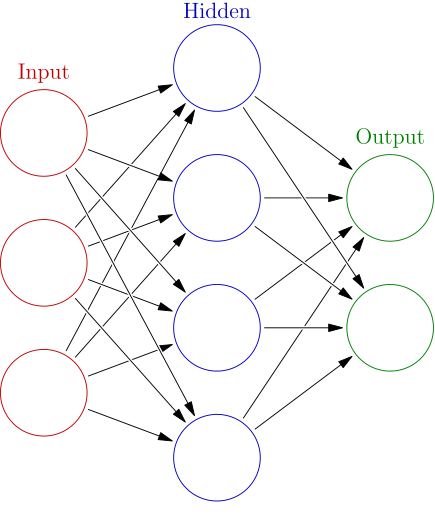
\includegraphics[width=0.38\textwidth]{images/Colored_neural_network.svg.png}
  \caption{Fully connected feed-forward neural network}
  \label{fig:wrapped}
\end{wrapfigure}
	
	
	It is important to mention that there are different architectures of neural networks two of which we will explore in more detail in the section Long Short-Term Memory (LSTM) and Convolutional Neural Network (CNN). They can vary heavily in their functionality, use cases and structure. A common fully connected feed forward neural network is what we look at now.\\
	
	This basic neural network has one input and one output layer. In addition to those the network can consist of an arbitrary number of hidden layers between input and output layer. Each layer including input and output layer consists of at least one neuron. The number of neurons in the input layer needs to match the size of our input. The input necessarily consists of one or more values. So, if our neural network takes images of pixel size (28 x 28) as input then we have 784 values per image and need 784 neurons in the input layer. The fact that the number of neurons in the input layer needs to match the size of the input applies particularly to this feed forward neural network. We will later see that for example a convolutional neural network has a different way of dealing with the input size. \\
	
	Each neuron is connected with other neurons. These connections are defined by their weight. In our fully connected feed forward neural network every neuron has a connection to every neuron of the next layer. Again, this is just the case for our standard fully connected feed forward neural network. There exist more specialized structures for which this rule doesn’t apply. The value of a neuron is fed forward to all other neurons it has a connection to. In our basic case the neurons only have connections to neurons of the next layer so the values only move from left to right as the directed arrows between the neurons in the image suggest. When a value is fed forward it is multiplied by the weight of the connection. A neuron receives one weighted value per neuron that has a connection to it. Within the neurons all these weighted values are added up and the bias of the neuron is added. The value of the bias is stored inside the neuron and it is learned during training. Before the value is given forward to the next neurons, a function is applied. This happens in each neuron. The function is called activation function. It has its name because the function is what decides whether a neuron is “activated”.\\
	\subsubsection{Activation Functions}
	This is very much inspired by nature. The neurons in our brains receive an input which arrives as electrical signals. Only when the membrane potential exceeds a certain threshold does the neuron “fire” an action potential. Artificial neural networks simulate this behavior with an activation function which also is designed to decide whether and how strong a neuron “fires”. One widely used activation function is called Rectified Linear unit (ReLU). We can see the graph of the ReLU function in Figure 5.2.
	
\begin{figure}[H]
  \centering
  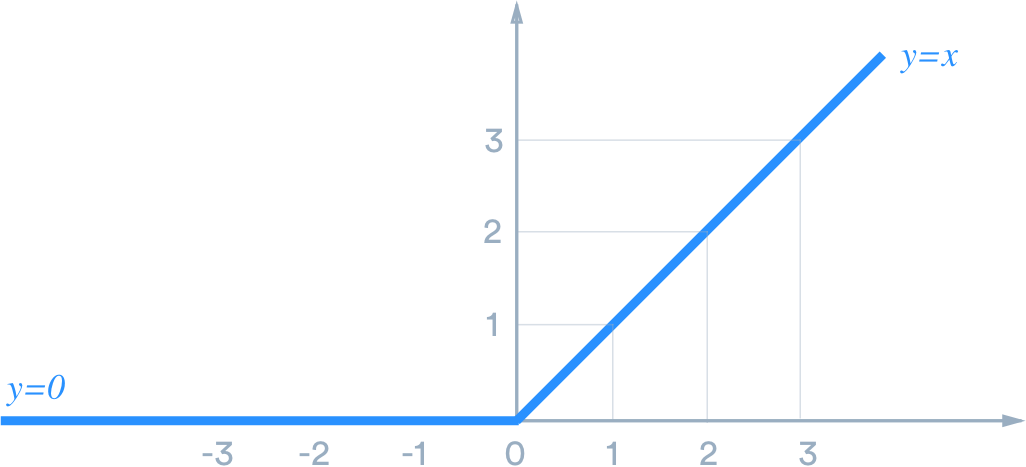
\includegraphics[width=\textwidth]{images/ReLU.png}
  \caption{ReLU activation function}
  \label{fig:fullwidth}
\end{figure}
	
	It “rectifies” or cuts off the negative part and sets every value in it to zero. Every value greater than or equal to zero is retained by a linear function. That's a very simple understanding of the activation behavior.
	\subsubsection{Non-linearity}
	We need to introduce the concept of non-linearity here. A linear relation between two variables x and y always has this structure:
\begin{equation}
y = a x + b
\end{equation}
Linear functions let us solve linear problems. They always are a straight line when drawn as a graph. For example, the relation of euros to cents is a linear function. You always multiply the amount of euros by 100 to get the number of cents that have the same worth.\\
A nonlinear relationship between two variables is every relationship but a linear relationship. All of those functions are nonlinear. 
\begin{equation}
f(x) = |x|,\quad f(x) = x^2,\quad f(x) = \sin(x)\,.
\end{equation}

If we want to model nonlinear relationships, we need a nonlinear function to do that. One example that actually fits nicely to the stock market is compound of interest. If you want to model the course of an investment given a certain interest rate greater than zero, you are facing a nonlinear problem which is only solvable with a non-linear function. \\
In the fewest cases the problem we want to solve using a neural network is linear. More precisely we usually don’t know the exact relation between the input and output data which is exactly why we are applying a machine learning algorithm to learn it. We have to assume nonlinearity. Even in the case that the relation is perfectly linear, then we can still use nonlinear functions since they can also model linear relations.\\
\\\
Let’s assume we are having only linear activation functions which is the case that includes having no activation function at all because simply passing on the values would be synonymous to the identity function which is a linear function. Then our whole neural network would only be able to capture linear relationships between input features and the output. This is due to the nature of stacked linear functions. If you stack n linear functions, then no matter how big n is, the resulting function always collapses down to a linear function with n input variables. We look at a simple example that illustrates that.
\begin{enumerate}
  \item First function $f_{1}$ operates on input variable $x$:\hfill
    $\displaystyle f_{1}(x)=a_{1}x+b_{1}$

  \item Second function $f_{2}$ operates on input variable $y$:\hfill
    $\displaystyle f_{2}(y)=a_{2}y+b_{2}$

  \item Third function $f_{3}$ operates on input variable $z$:\hfill
    $\displaystyle f_{3}(z)=a_{3}z+b_{3}$
\end{enumerate}

When we stack the functions:
\begin{align*}
  f_1\bigl(f_2(f_3(z))\bigr)
  &= f_1\bigl(f_2(a_3 z + b_3)\bigr)
   = f_1\bigl(a_2\,(a_3 z + b_3) + b_2\bigr)\\
  &= a_1\bigl(a_2\,(a_3 z + b_3) + b_2\bigr) + b_1\\
  &= a_1\bigl(a_2 a_3\,z + a_2 b_3 + b_2\bigr) + b_1\\
  &= a_1 a_2 a_3\,z \;+\; a_1 a_2 b_3 + a_1 b_2 + b_1.
\end{align*}

Since \(a_1,a_2,a_3,b_1,b_2,b_3\) are fixed constants from the linear functions, we can compute them together to their effective values.
\begin{equation}
  W_{\mathrm{eff}} = a_1\,a_2\,a_3,
  \qquad
  b_{\mathrm{eff}} = a_1a_2b_3 + a_1b_2 + b_1,
\end{equation}
The resulting function is:
\begin{equation}
  f_4(z) = W_{\mathrm{eff}}\,z + b_{\mathrm{eff}}.
\end{equation}
This shows that no matter how many layers of purely linear neurons you stack, you end up with a single affine map—and thus can never capture any nonlinear relations between input and output.  That is why neural networks require nonlinear activation functions (e.g.\ ReLU) between layers. \\

We talked about the connections between the neurons and we understood that these connections are defined by their weight. The weights which are stored in the connection and the biases which are stored in the neuron are learned during training through backpropagation. The weights, biases and the concrete architecture, so the number of neurons per layer the number of layers and the activation functions, is what constitutes the knowledge of the network. With this information you can reconstruct the network with its current knowledge state. 
	\subsubsection{weights and biases}
	We talked about the connections between the neurons and we understood that these connections are defined by their weight. The weights which are stored in the connection and the biases which are stored in the neuron are learned during training through backpropagation. The weights, biases and the concrete architecture, so the number of neurons per layer the number of layers and the activation functions, is what constitutes the knowledge of the network. With this information you can reconstruct the network with its current knowledge state. 
	\subsubsection{backpropagation}
	To understand the concept of backpropagation we will walk through the process of one prediction using an example network. One prediction or the process of walking the input from the input layer through the network to the output layer is called forward propagation. \\
	We can see the example neural network we use for this purpose drawn in Figure 5.3.
	
	
\begin{figure}[htbp]
  \centering
  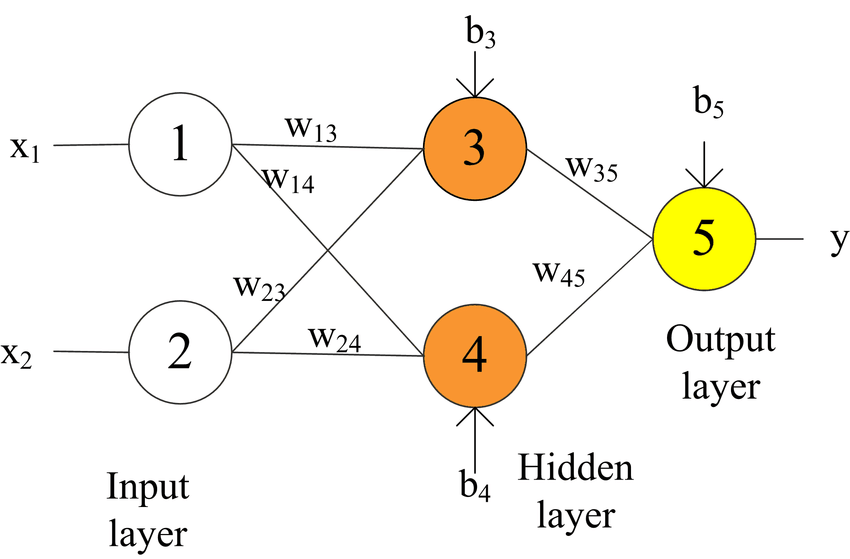
\includegraphics[width=\textwidth]{images/Neural_Network.png}
  \caption{Example neural network}
  \label{fig:fullwidth}
\end{figure}








\noindent
Where..:\\\\
\medskip
\begin{tabular}{@{}l@{\,--\,}l}
  $x_1$       \hspace*{2em} & \hspace*{2em} is the input feature~1 \\
  $x_2$       \hspace*{2em} & \hspace*{2em} is the input feature~2 \\
  1,2,3,4,5   \hspace*{2em} & \hspace*{2em} are the neuron indices (layer nodes) \\
  $b_n$       \hspace*{2em} & \hspace*{2em} is the bias of neuron~$n$ \\
  $w_{ij}$    \hspace*{2em} & \hspace*{2em} is the weight of the connection from neuron~$i$ to neuron~$j$ \\
  $y$         \hspace*{2em} & \hspace*{2em} is the output value
\end{tabular}\\

	
	
One forward propagation results in an output. If you have labeled training data and labeled outputs for each input, then you can compare the predicted value with the actual value to learn better weights and biases that lead to more accurate predictions. We will first only do the process of one forward propagation and then show how the network refines its weights and biases comparing the predicted value with the actual one.\\\\

	
\noindent\underline{Example:}\\

\noindent
$X1 = 1.0$ \\
$X2 = 2.0$ \\
Value in neuron 1 = 1.0 \\
Value in neuron 2 = 2.0 \\
$w_{1,3} = 0.5$; $w_{2,3} = 0.9$; $b_3 = 0.5$ \\
$w_{1,4} = 0.3$; $w_{2,4} = -0.4$; $b_4 = 0.6$ \\
$w_{3,5} = 0.7$; $w_{4,5} = 0.3$; $b_5 = 0.8$ \\[1em]
\noindent
The activation function in neuron 3 and 4 is ReLU. The output layer has no activation function and the input layer neither has an activation function because it just contains raw input.\\\\
The proccessing order is:

\begin{enumerate}
  \item Value $x_1$ and $x_2$ simply arrive in neuron 1 and 2.
  \item Neuron 3 receives two values and together with its bias $b_3$ adds them up.\\\\
  $x_3 = x_1 \cdot w_{1,3} + x_2 \cdot w_{2,3} + b_3$ \\
  $x_3 = 1.0 \cdot 0.5 + 2.0 \cdot 0.9 + 0.5 = 2.8$\\
  So the weights are multiplied with the transported value and added together with the bias from the neuron.\\
  Now the activation function is applied on 2.8: \\
  $x_3 = \max(0, 2.8) = 2.8$
  
  \item Neuron 4 receives two values and together with its bias $b_4$ adds them up.\\\\
  $x_4 = x_1 \cdot w_{1,4} + x_2 \cdot w_{2,4} + b_4$ \\
  $x_4 = 1.0 \cdot 0.3 + 2.0 \cdot (-0.4) + 0.6 = 0.1$\\
  Now the activation function is applied on 0.1: \\
  $x_4 = \max(0, 0.1) = 0.1$
  
  \item Neuron 5 receives two values and together with its bias $b_5$ adds them up.\\\\
  $x_5 = x_3 \cdot w_{3,5} + x_4 \cdot w_{4,5} + b_5$ \\
  $x_5 = 2.8 \cdot 0.7 + 0.1 \cdot 0.3 + 0.8 = 2.79$
  
  \item The calculated output $y$ is 2.79
\end{enumerate}
\noindent
Our calculated output $y$ with 2.79 is what our neural network predicts as output for the input $x_1 = 1.0$ and $x_2 = 2.0$. Let’s now assume that the actual output value for this input is 2.1. We can calculate the loss and perform a backpropagation.\\\\
\noindent
The loss $E$ is calculated as:

\begin{equation}
E = \frac{1}{2}(y - t)^2
\end{equation}

\noindent
Where..:\\\\
\medskip
\begin{tabular}{@{}l@{\,--\,}l}
  $E$         \hspace*{2em} & \hspace*{2em} is the loss \\
  $y$         \hspace*{2em} & \hspace*{2em} is the predicted outcome \\
  $t$         \hspace*{2em} & \hspace*{2em} is the actual outcome \\
\end{tabular}\\
\
In our case that’s:

\[
E = \frac{1}{2}(2.79 - 2.1)^2 = \frac{1}{2}(0.69)^2 = \frac{1}{2}(0.4761) = 0.23805
\]

In order to now perform backpropagation, we need to calculate the derivates of the loss function in respect to the weights.\\\\
	
	
	
	
	
	
	
	
	
	
	
	
	
	
	
	
	
	
	
	
	
	
	
	
	
	
	
	
	
	
	
	

The structure we just looked at is a very basic version of a neural network. It illustrates all basic mechanisms of modern feed forward neural networks. In practice depending on the concrete architecture, they can be much more complex with many hidden layers and many more neurons per layer. Especially the LSTM network has a remarkable architecture and we will look at it in this section.
	
	\subsection{Recurrent Neural Networks}
	One example of these modified neural networks are recurrent neural networks (RNNs). They are designed for and applied to context sensitive problems such as speech, audio or video processing and time series forecasting. RNNs are able to store the context of a sequence. if you for example read a sentence, then in order to make sense of the end of this sentence you need to remember the beginning of it or at least the key context of the previous words. The same is the case for video data. If you want to understand what is going on in a video clip you cannot just look at the last frame. Instead, you need to look at the whole clip frame after frame while remembering key information from previous frames to understand its content. That’s basically what RNNs are capable of. They can store the context from previous parts of a sequence and use this context to perform predictions or classifications. That’s why the input of an RNN is not one set of values but instead a sequence of sets of values. We call these sets time steps right now. These time steps are fed into the RNN one after another. After every time step the network stores a hidden state vector. In the base case this hidden state vector captures one value or hidden state for each hidden neuron. Hidden neurons are neurons in hidden layers. These hidden states are stored until the next time step and simply passed as normal values to other neurons. The input for the RNN has the size of the data of one-time step. In the case of a video, it would most likely be the size of one frame. When we feed the first frame into the RNN, a hidden state vector is produced. When we move on to the next frame then the neurons receive this next frame as input and in addition to that the hidden state vector that was produced from the previous frame. Like that the network stores contextual information across time steps and always processes the current input data taking into account peculiarities or patterns from previous time steps. In the case of stock price forecasting one time step is one period for which we have input feature values. In our specific context we will have daily stock data so one time step is equivalent to one day of stock data.\\
	We can see how an RNN can look like illustrated in Figure 5.4. 
	
	\begin{figure}[htbp]
  \centering
  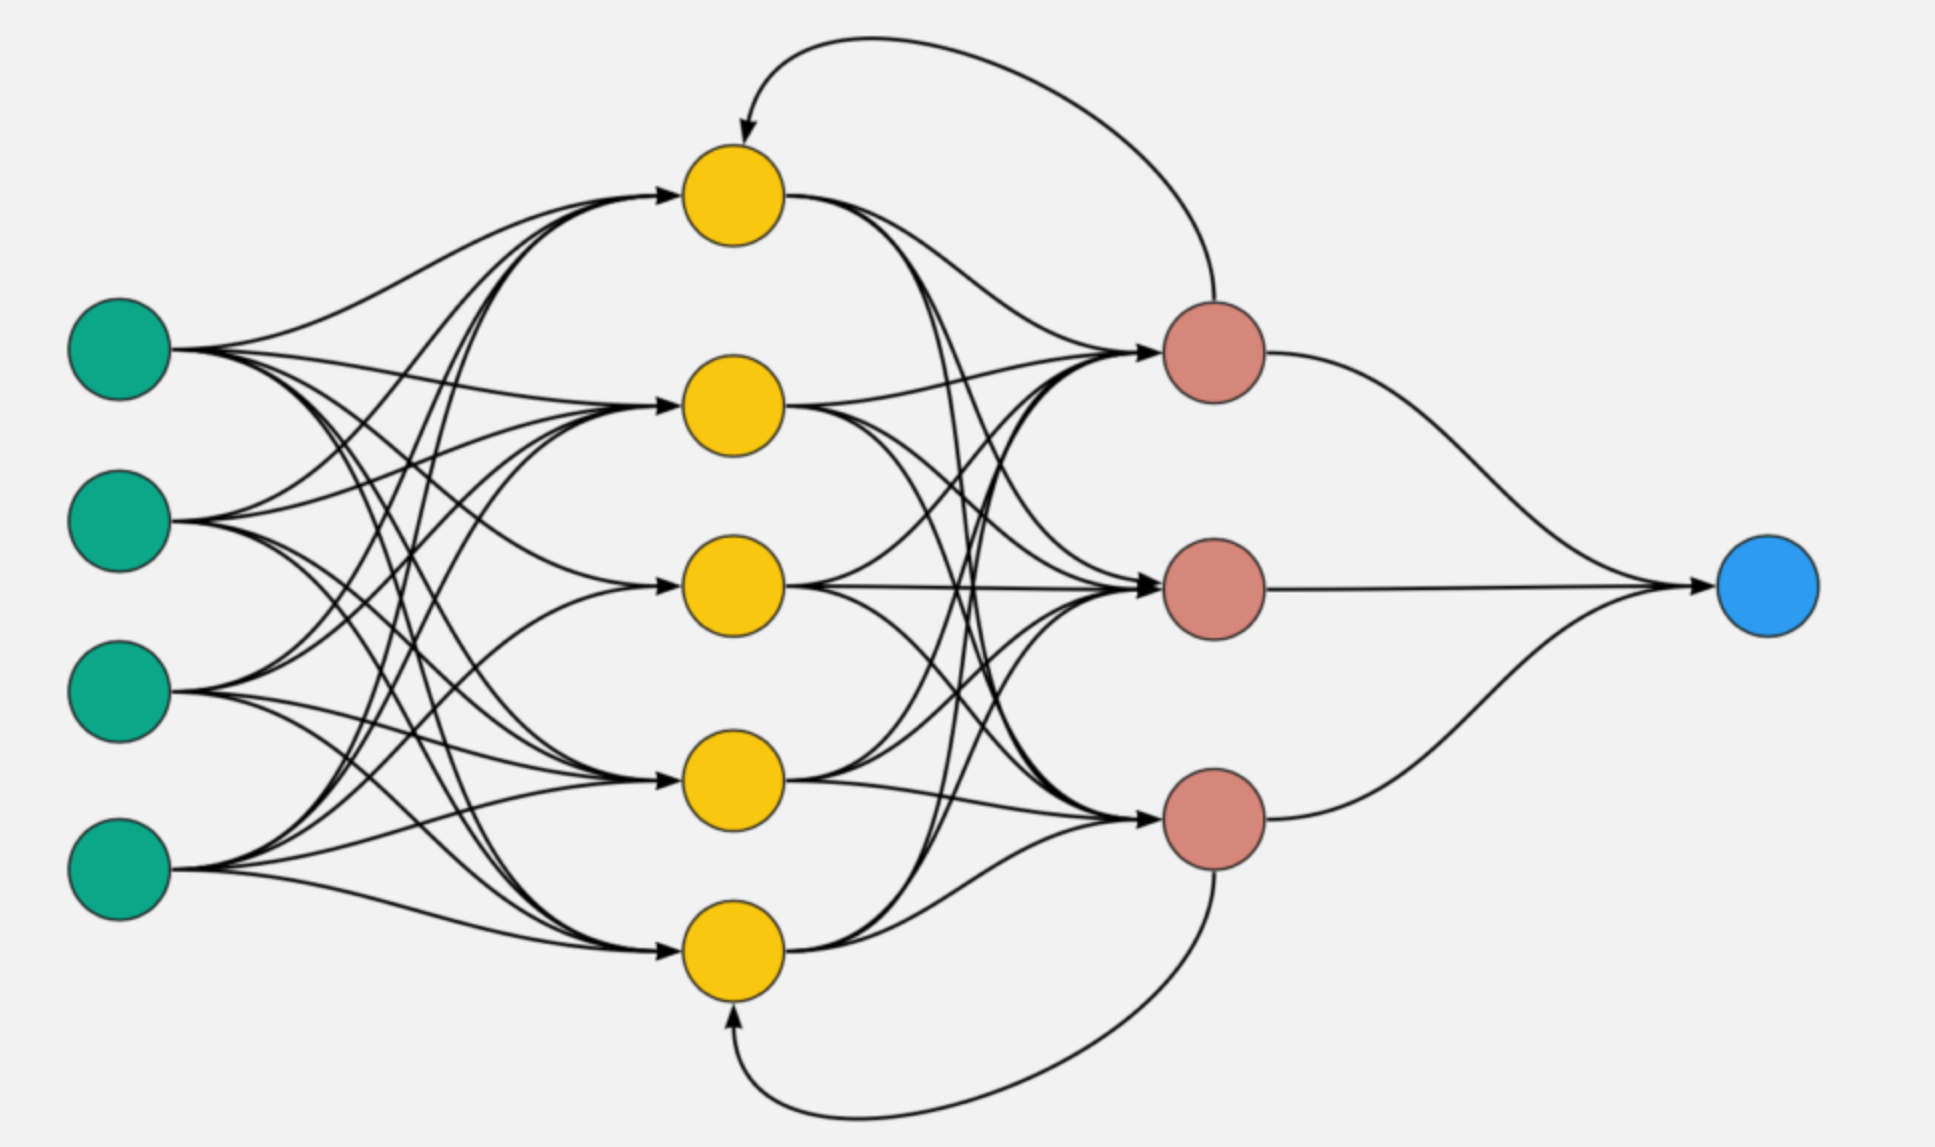
\includegraphics[width=\textwidth]{images/RNN.png}
  \caption{RNN}
  \label{fig:fullwidth}
\end{figure}
	
	
	In that case the green neurons are our input layer, so we know that our input consists of 4 values or in other words each time step carries 4 values as input. We have two hidden layers which are the yellow and the red neurons and we have an output layer which consists of the blue neuron, which means the network computes one output value. All arrows that are directed from left to right symbolize connections used during one forward propagation. The arrows from the first and third red neuron are directed to the left which means they constitute the hidden state vector. At time step t we feed the 4 input values which are represented by the green neurons into the network. We perform a forward propagation as we learned before with one exception. the output value that the first and third red neuron produce at this time step t is stored inside the hidden state vector. When we are done with this forward propagation, we feed the 4 input values from the next time step t+1 into the network. We do that by assigning the input values to the 4 green input neurons. We again perform a simple forward propagation with the difference that we feed the stored hidden states from the previous time step t into the two yellow neurons according to the arrows.\\
	The process of backpropagation hereby works similar to how it works in the feed forward neural network that we looked at earlier with the difference that we backpropagate through the time steps. To do so, we would unroll the network along its time steps. Like that we end up with long chains of derivatives for the single weights and biases. The more time steps we have the longer these chains of derivatives are. We skip looking at a concrete example here, because in its core functionality it is similar to the back propagation we learned before. \\
	The main thing to keep in mind for RNNs is that they can interpret input data in the context of previous input data. They do that by storing key information from previous time steps in a vector that is stored until the next time step.
	
	\subsubsection{Long Short-Term Memory (LSTM)}
	One concrete architecture of recurrent neural networks are Long Short-Term Memory networks. Beyond feeding output values to the next time step, LSTM networks use different gates to facilitate the storing of context specific states. An LSTM network also consists of layers. The greatest difference to other neural networks is that the LSTM cells or units have built in mechanisms to maintain safe states. Furthermore, LSTM layers always consist of one LSTM cell that serves as multiple units of that by storing one value for each unit in the form of a state vector. There is one cell per layer but it behaves as many units since it processes a number of input values from the input vectors parallel with separate weights per units. There are two state vectors that are maintained by the LSTM network, a cell state and a hidden state. The cell state vector is only passed across time steps and serves as input to the same cell for the next time step. The other state vector is the hidden state which is also passed to the same cell in the next time step and except for the first layer which receives the raw input, every following layer receives the hidden state from the previous layer as input. So, we have the cell state vector and the hidden state vector.
	
	
In figure 5.5 we can see how the LSTM cell processes the input. The equations for the gates, the outputs and the inputs are described below to understand how the LSTM cell computes the values. z(t) is defined as a combined vector that simply concatenates the input x(t) and the previous hidden state h(t-1). The LSTM network stores weight and bias matrices. It stores one array of weights per gate and per unit so every gate in every unit has its own weight array which has the size of the input vector z(t) and carries one weight per input element of z(t). The bias matrices hold biases for each gate for each LSTM unit but they are the same for all input elements, so the same bias is added to every element of the combined input vector z(t) in one gate of one unit. The sigmoid and tanh activation functions are applied as part of the gates to introduce non-linearity to the model. We understood why non-linearity is an important concept for Machine Learning.	
	
	
	
\begin{figure}[htbp]
  \centering
  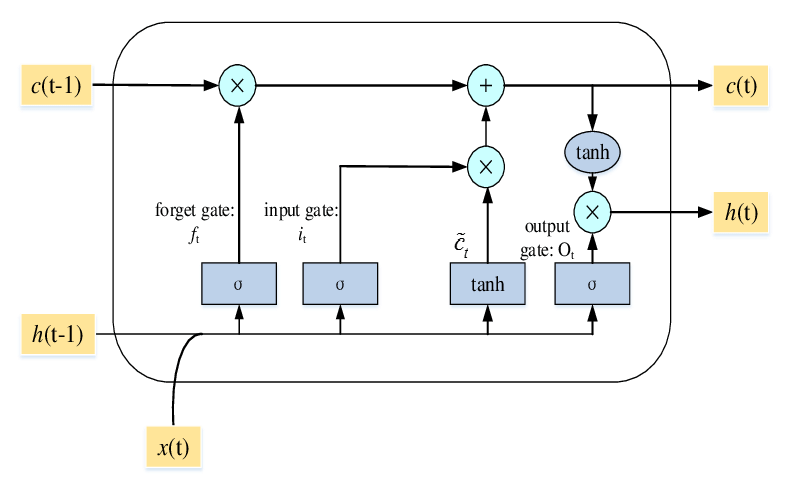
\includegraphics[width=\textwidth]{images/LSTM.png}
  \caption{LSTM cell}
  \label{fig:fullwidth}
\end{figure}

	
	
\begin{minipage}{\textwidth}
	The input..:\\
\medskip
\begin{tabularx}{\textwidth}{@{}l@{\hspace{2em}--\hspace{2em}}X@{}}
  $c(t-1)$ & is the cell state from the same cell from the previous time step. \\
  $h(t-1)$ & is the hidden state from the same cell from the previous time step. \\
  $x(t)$   & is the input which is the raw input for the first LSTM layer and the hidden state from the previous layer for every layer which is not the first layer. \\
\end{tabularx}


\end{minipage}

\begin{minipage}{\textwidth}

	and the output..:\\


\begin{tabularx}{\textwidth}{@{}l@{\hspace{2em}--\hspace{2em}}X@{}}
  $c(t)$ & is the new cell state which will be the input for the same cell in the next time step. \\
  $h(t)$ & is the new hidden state which will be the input for the same cell in the next time step and for the next layer. \\
\end{tabularx}\\
\end{minipage}

\begin{minipage}{\textwidth}

The following equations are used to calculate the output by applying the gates.
\[
\begin{aligned}
  i(t) &= \sigma \big( W_i z(t) + B_i \big)  && \text{(input gate)} \\
  f(t) &= \sigma \big( W_f z(t) + B_f \big)  && \text{(forget gate)} \\
  o(t) &= \sigma \big( W_o z(t) + B_o \big)  && \text{(output gate)} \\
  \tilde{c}(t) &= \tanh \big( W_c z(t) + B_c \big) && \text{(cell input activation)} \\
  c(t) &= f(t) \odot c(t-1) + i(t) \odot \tilde{c}(t) && \text{(new cell state)} \\
  h(t) &= o(t) \odot \tanh \big( c(t) \big) && \text{(new hidden state)} \\
\end{aligned}
\]

\end{minipage}
\medskip
\begin{minipage}{\textwidth}
The activation functions, weights and biases matrices are:\\

\begin{tabularx}{\textwidth}{@{}l@{\hspace{2em}--\hspace{2em}}X@{}}
  $B_i$      & the bias vector for input gate \\
  $B_f$      & the bias vector for forget gate \\
  $B_o$      & the bias vector for output gate \\
  $B_c$      & the bias vector for cell input activation \\
  $W_i$      & the weight matrix for input gate \\
  $W_f$      & the weight matrix for forget gate \\
  $W_o$      & the weight matrix for output gate \\
  $W_c$      & the weight matrix for cell input activation \\
  $\sigma(\cdot)$ & the sigmoid activation function \\
  $\tanh(\cdot)$  & the hyperbolic tangent activation function \\
\end{tabularx}\\\\
\end{minipage}

In relation to the basic neural network, which we looked at in the beginning, the LSTM has only one cell per layer but still processes vectors, so it processes a multivariate input. It also differs by maintaining certain safe states to capture context or past events. That make it very suitable and strong in solving time series problems and it is the reason it was observed to perform very well in stock price forecasting.\\
In practice the LSTM layers are often followed by fully connected layers that make predictions out of the learned patterns. That is not technically necessary, because the final hidden state vector can also serve as output but in case the output needs to be further classified or put into a different shape one or more fully connected layers help with that.



	
	\subsection{Convolutional Neural Networks}
	Another type of neural networks is a Convolutional Neural Network (CNN). These are explicitly performant with spatial data, for example images. That is because they detect local patterns and maintain spatial relation of the input data. To understand what that means we look at how CNNs function. Throughout our explanation we understand their functionality in general and after that we discover how they can be applied to time series data. \\

	CNNs mainly consist of three different types of layers:
\begin{itemize}
  \item Convolutional Layer
  \item Pooling Layer
  \item Fully-Connected Layer
\end{itemize}
A series of convolutional and pooling layers usually is supposed to extract important features from the input in an efficient and generalized way, while fully-connected layers afterwards make sense of the extracted features and create predictions or classify the input depending on the use case.

	\subsubsection{Convolutional layer}
	The first layer of the network typically is a convolutional layer. It receives a 3D input tensor. In the case of an image that is (height(pixels) * width(pixels) *channels (color channels)). The convolutional layer is mainly defined by its parameters for which:\\
\begin{tabularx}{\textwidth}{@{}l@{\hspace{2em}--\hspace{2em}}X@{}}
  Number of filters & is the number of filters that are applied to the input of that layer \\
  Kernel size       & is the size of the filters which are applied \\
  Stride            & is the step size with which the filters slide over the input \\
\end{tabularx}
	
	
	There are more parameters with which you can further define the nature of the layers. We explain them in more detail in the section hyperparameter tuning but for now we only need to understand those three parameters.\\
	
The convolutional layer applies filters on the input. These filters are supposed to extract information about the occurrence of certain patterns. 3x3xchannels or 5x5xchannels is the typical shape of these filters but while they usually have the number of channels as one dimension, they can have any size for the other two dimensions. The filters are tensors themselves that carry one value in each cell. When a filter is applied to an input it slides over the input with a step size which is defined as the stride parameter. A stride of one means the filter moves one cell per step. We said that the filter slides over the input. That means that the filter overlaps with certain cells of the input. In a position in which two cells overlap, the values of the two cells that overlap, one from the input and one from the filter are multiplied together and the products of all overlaps at one filter position is summed up. Applying one filter results in one feature map. The summed-up values of one position of a filter are part of the value for the cell of the feature map at that position. So, applying a filter at one position results in one value in the feature map. After applying the filter, a bias value is added to the resulting value. Every cell in a feature map gets added the same bias so there is one bias per filter. In that way we apply all filters of the convolutional layer and end up with one feature map for each filter. The idea behind the feature maps is that the filters have values in their cells in an order which, when multiplied with the input result in a large total sum in case they detect the pattern which is described by that specific order of elements in the filter. A large sum in that case means that a strong occurrence of the pattern encoded in the filter is detected at that position. One feature map now tells us for each position how strong the feature that it is designed to detect occurs at that position. After applying all filters, we end up with one feature map per filter. \\

\begin{figure}[htbp]
  \centering
  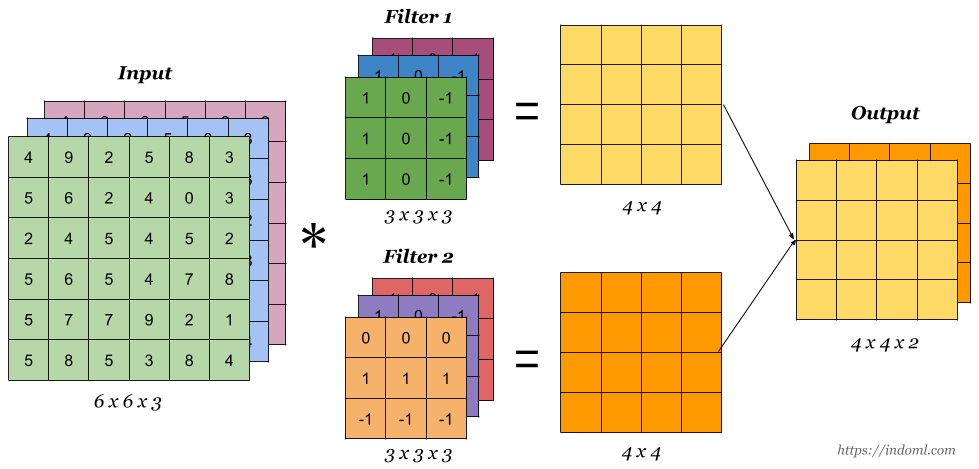
\includegraphics[width=\textwidth]{images/CNN_filters.png}
  \caption{First convolutional layer}
  \label{fig:fullwidth}
\end{figure}

Figure 5.6 illustrates one example for that. We see our input on the left which seems to be an RGB image and we see two filters that have weights or values for every cell in every color channel. Unfortunately, we can only see the upper most channel in the image now so we only apply the upper most channel of the filter to the upper most channel of the input. Actually, at one position, every channel of the filter would be applied to the input or in other words to the according channel of the input and then the total sum of all filters constitutes the value for the one cell in the feature for that position but we only look at the upper most channel \cite{51}.\\
	
We can see, that the green filter would result in the highest possible value if the cells on the left side are as big as possible while the cells on the right side of the filter are as close to zero as possible since they will be subtracted and the values on the left will be added. So, the spatial feature this filter could be looking at could be a vertical edge with low color levels in its right side but this is just a hypothetical interpretation to understand how these filters work.\\
	
In the following starting with figure 5.7, we see a series of images that illustrate how the filters are applied, how the bias is added and how the activation function is applied.
\begin{figure}[htbp]
  \centering
  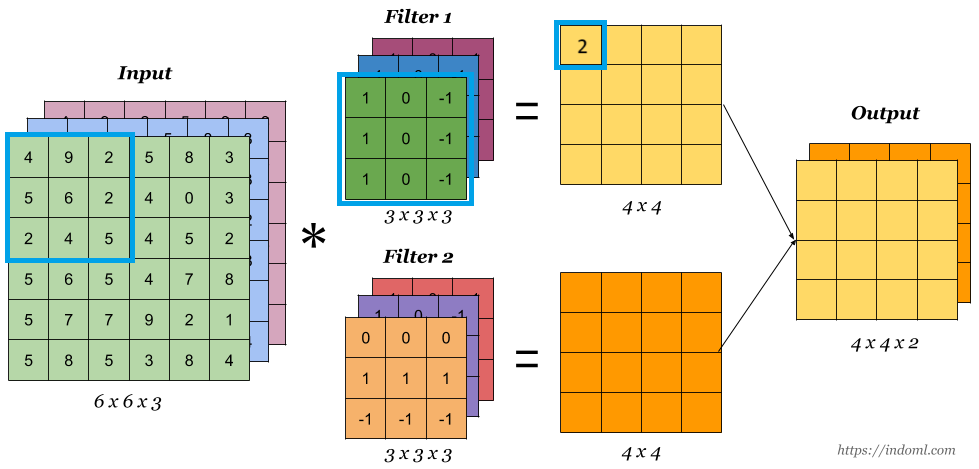
\includegraphics[width=\textwidth]{images/CNN_filters_0.png}
  \caption{Applying the convolutional filter 1}
  \label{fig:fullwidth}
\end{figure}
	
\begin{figure}[htbp]
  \centering
  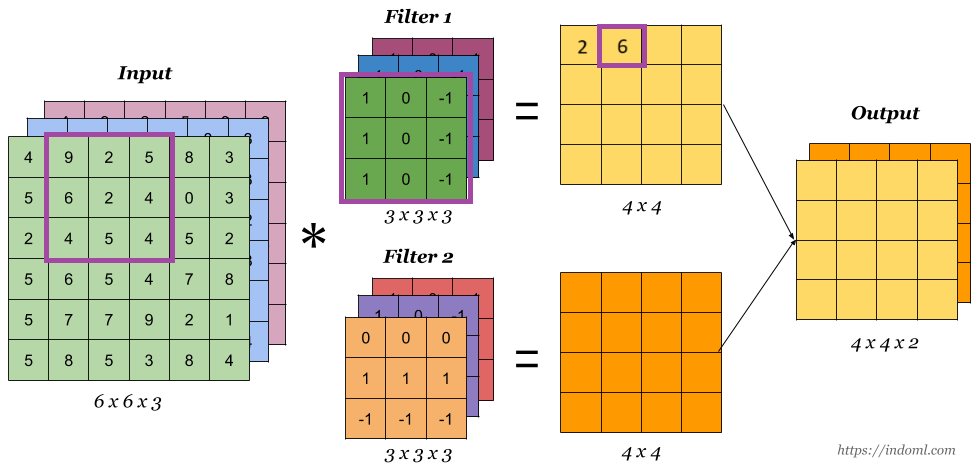
\includegraphics[width=\textwidth]{images/CNN_filters_1.png}
  \caption{Applying the convolutional filter 2}
  \label{fig:fullwidth}
\end{figure}

\begin{figure}[htbp]
  \centering
  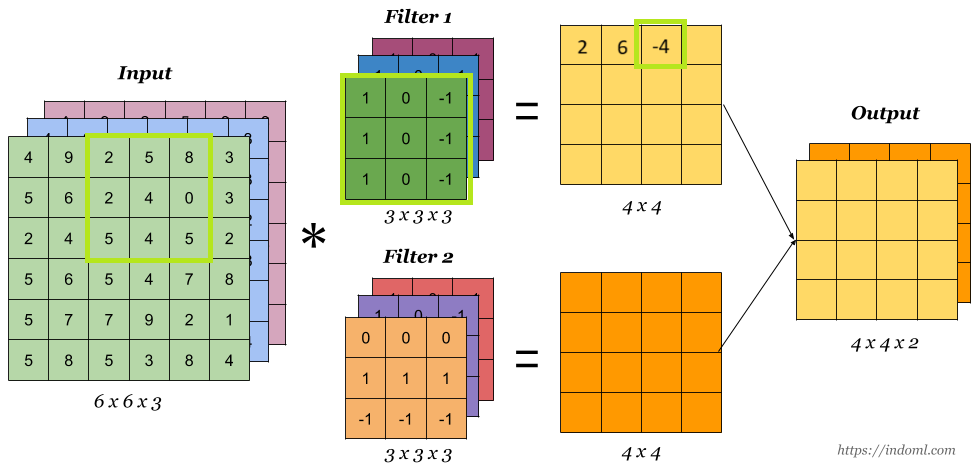
\includegraphics[width=\textwidth]{images/CNN_filters_2.png}
  \caption{Applying the convolutional filter 3}
  \label{fig:fullwidth}
\end{figure}

\begin{figure}[htbp]
  \centering
  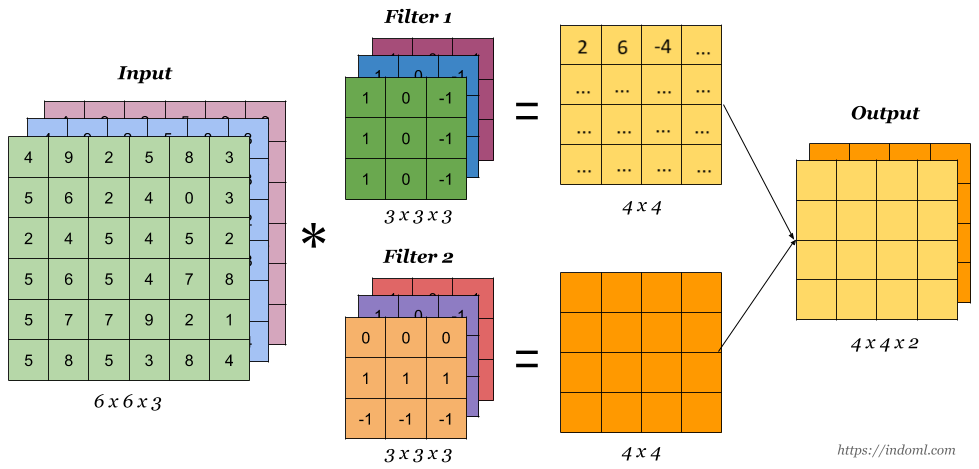
\includegraphics[width=\textwidth]{images/CNN_filters_3.png}
  \caption{Applying the convolutional filter to the remaining positions}
  \label{fig:fullwidth}
\end{figure}
\FloatBarrier
Like that the filter is applied and the feature map is constructed. The next step is to add the bias for each cell in the feature map. We simply assume a bias of 2.

\begin{figure}[htbp]
  \centering
  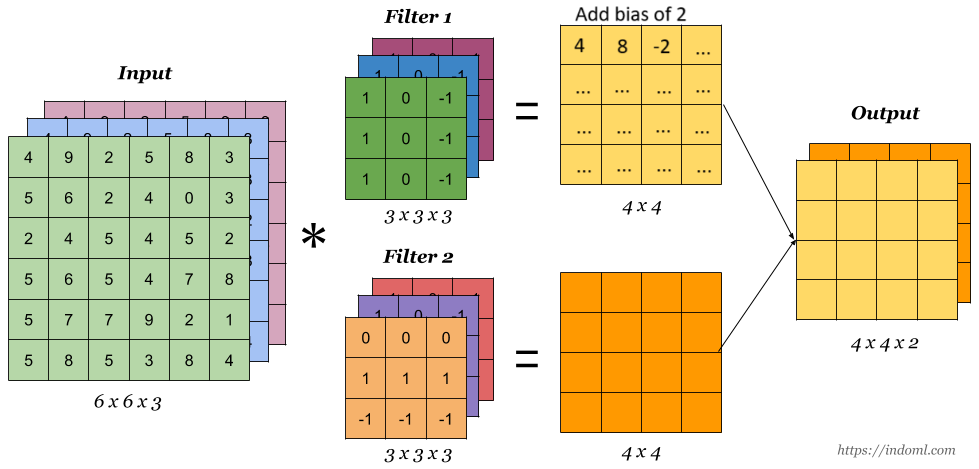
\includegraphics[width=\textwidth]{images/CNN_filters_3_5.png}
  \caption{Add a bias of two to every cell}
  \label{fig:fullwidth}
\end{figure}

\FloatBarrier
Right after adding the bias, we apply activation functions to the feature maps to introduce nonlinearity to the model. We looked at the importance of this concept earlier in this section. The activation function (e.g., ReLU) is simply applied to every cell of every feature map. 
\begin{figure}[htbp]
  \centering
  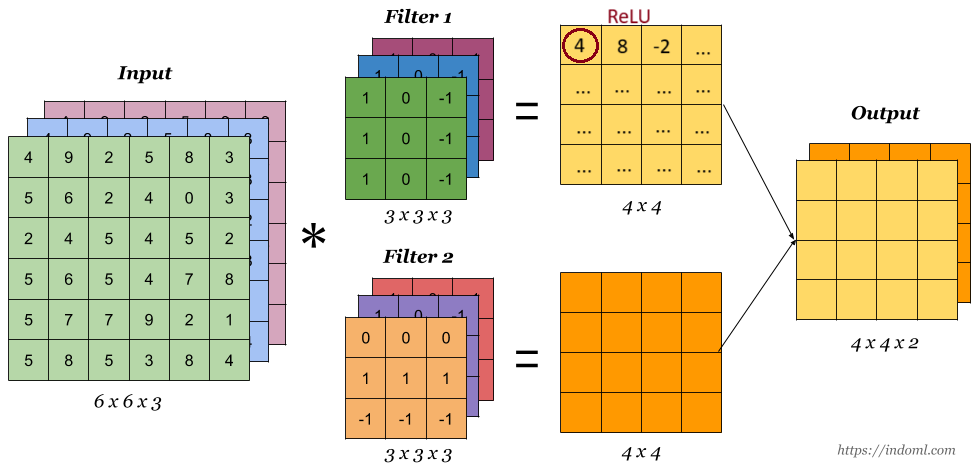
\includegraphics[width=\textwidth]{images/CNN_filters_4.png}
  \caption{Apply the activation function 1}
  \label{fig:fullwidth}
\end{figure}

\begin{figure}[htbp]
  \centering
  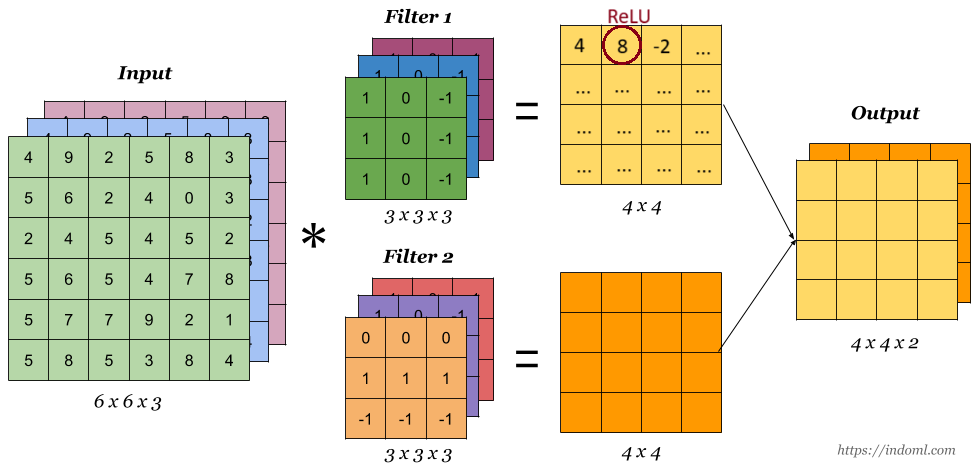
\includegraphics[width=\textwidth]{images/CNN_filters_5.png}
  \caption{Apply the activation function 2}
  \label{fig:fullwidth}
\end{figure}

\FloatBarrier
\begin{figure}[htbp]
  \centering
  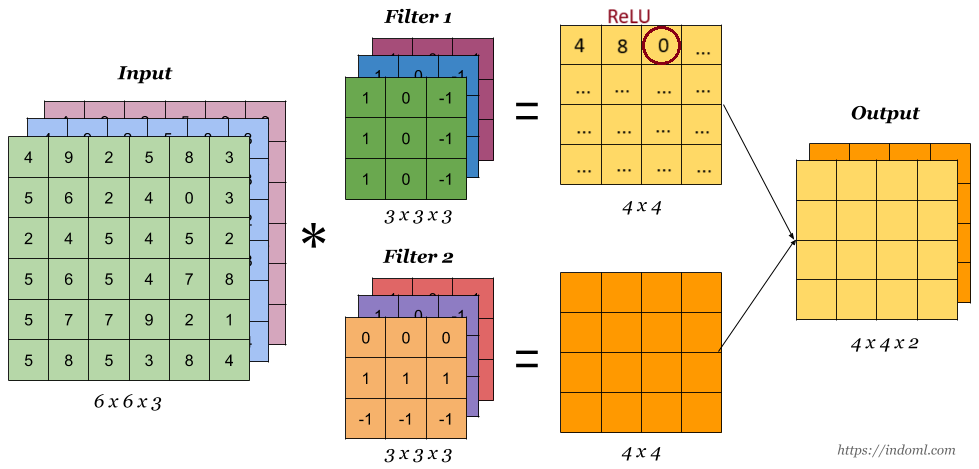
\includegraphics[width=\textwidth]{images/CNN_filters_6.png}
  \caption{Apply the activation function 3}
  \label{fig:fullwidth}
\end{figure}
	
\begin{figure}[htbp]
  \centering
  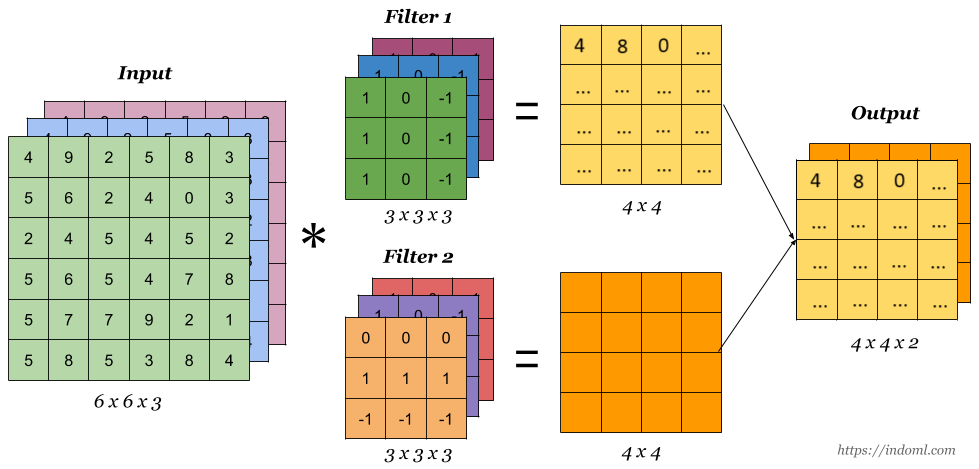
\includegraphics[width=\textwidth]{images/CNN_filters_7.png}
  \caption{Finalized feature map is part of the output}
  \label{fig:fullwidth}
\end{figure}
Like that we get the feature maps that will constitute the input channels for the next convolutional layer. But before we feed them into the next convolutional layer, we apply a pooling layer.
	
	
	
	\subsubsection{Pooling Layer}
	A convolutional layer is typically succeeded by a pooling layer. The pooling layer is designed to reduce the dimensions of the feature maps. This is an advantage for computational efficiency but it especially makes the model more robust. In the sense of an image, we can imagine it as reducing its resolution. We not just reduce the resolution randomly but instead we merge pixels while choosing to keep the most important information. The reason it makes the model more robust is that it filters out unnecessary information about the image and like that makes itself less susceptible to overfitting or noisy data. So, pooling is the process of down sampling the feature maps. One common approach for this is Max-Pooling. When Max-Pooling is performed we choose a frame size which is often 2 x 2. We move this frame over the original feature map and create a new feature map with reduced dimensions. For each position of the frame, we choose out of the 4 cells the highest value and take it as the new value that represents this square which the frame surrounds. Commonly a stride of 2 is used. That means we move the frame 2 cells to the right so that it captures the 2x2 square of cells next to our first one. We illustrate this concept in the following series starting with figure.
	
\begin{figure}[htbp]
  \centering
  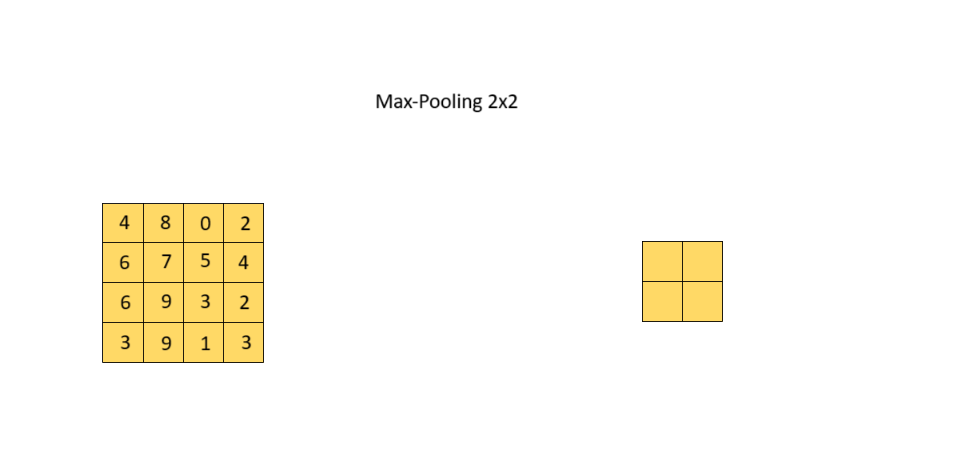
\includegraphics[width=\textwidth]{images/CNN_Max_Pooling_0.png}
  \caption{Max Pooling 1}
  \label{fig:fullwidth}
\end{figure}
	
\begin{figure}[htbp]
  \centering
  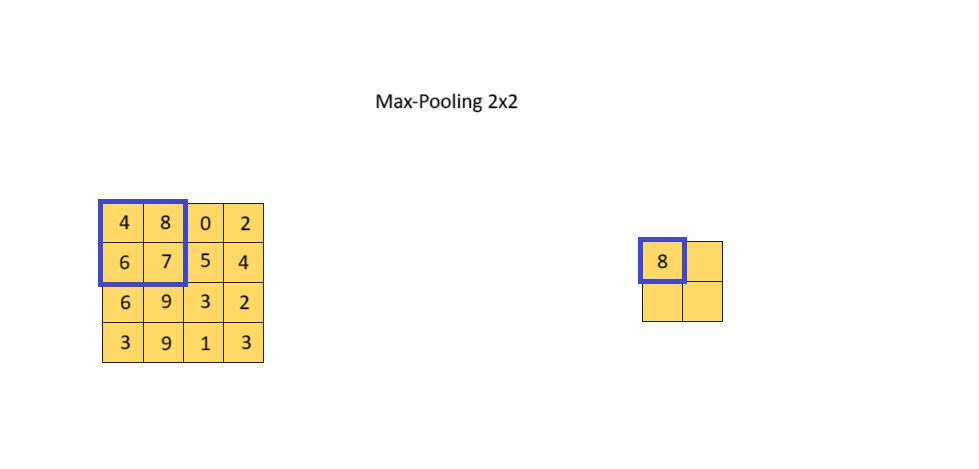
\includegraphics[width=\textwidth]{images/CNN_Max_Pooling_1.png}
  \caption{Max Pooling 2}
  \label{fig:fullwidth}
\end{figure}

\begin{figure}[htbp]
  \centering
  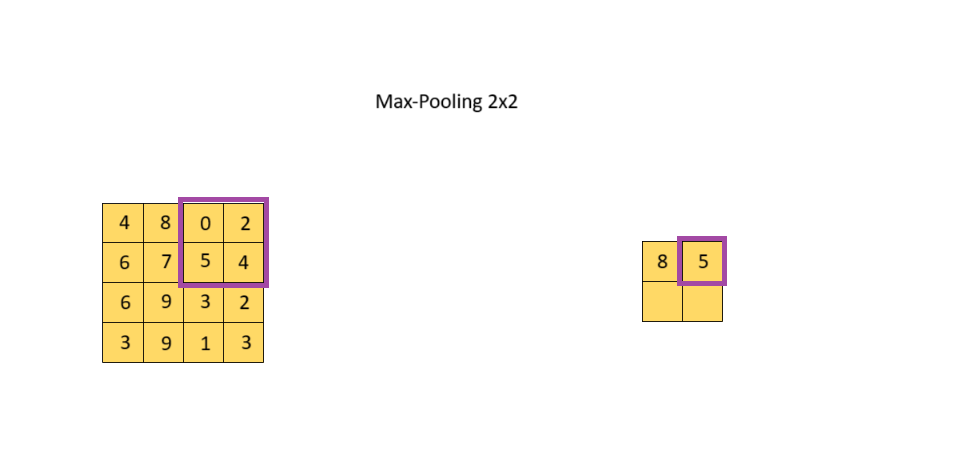
\includegraphics[width=\textwidth]{images/CNN_Max_Pooling_2.png}
  \caption{Max Pooling 3}
  \label{fig:fullwidth}
\end{figure}
\FloatBarrier
\begin{figure}[htbp]
  \centering
  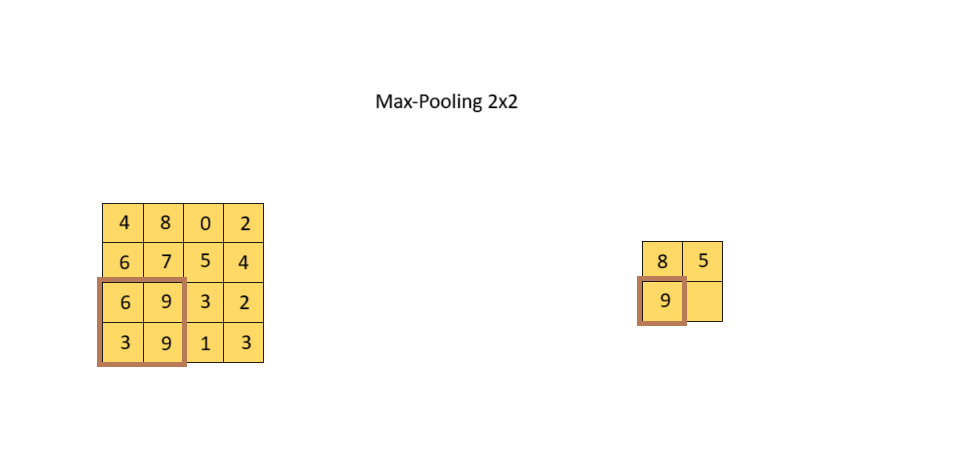
\includegraphics[width=\textwidth]{images/CNN_Max_Pooling_3.png}
  \caption{Max Pooling 4}
  \label{fig:fullwidth}
\end{figure}
	
\begin{figure}[htbp]
  \centering
  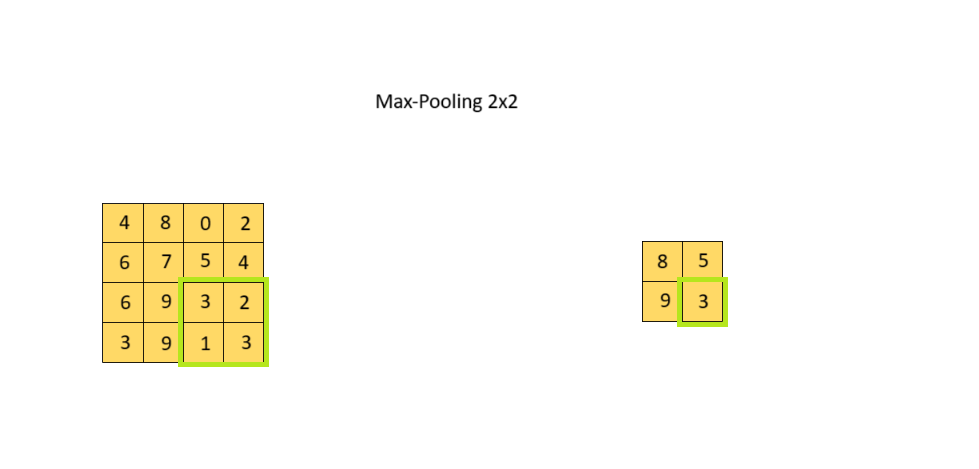
\includegraphics[width=\textwidth]{images/CNN_Max_Pooling_4.png}
  \caption{Max Pooling 5}
  \label{fig:fullwidth}
\end{figure}
	
	Like that we reduce the dimensions of the feature maps while we keep the most important information.
	
	\subsubsection{Viewed as a whole}
	
	This series of convolutional layer followed by a pooling layer can repeat a certain number of times. Each time more complex patterns can be detected. In the first convolutional layer we can only detect simple features such as edges, curves and maybe colors or other simple patterns. In the next convolutional layer, we apply again a certain number of filters but now the channels have changed. They changed from being the three-color channels of the original image to being maps that talk about occurrences of already more complex features in that image. That means the input is no longer the image itself but instead maps of extracted patterns from the image. That enables us to combine their occurrence to infer about the occurrence of even more complex patterns. \\
	This series of convolutional and pooling layers are followed by fully-connected layers which are fed the extracted features. Depending on the purpose of the network they apply a SoftMax function that takes the extracted features and creates probabilities of class membership that sum up to one. The whole process is illustrated below.
	
\begin{figure}[htbp]
  \centering
  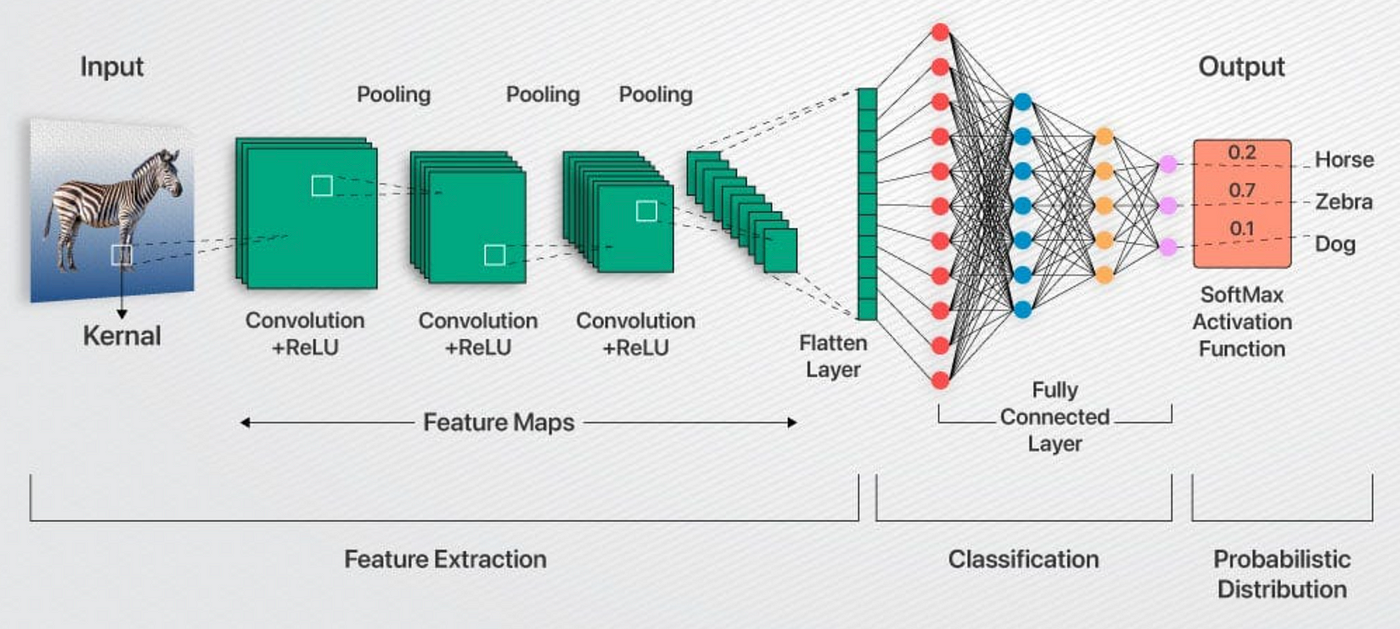
\includegraphics[width=\textwidth]{images/full_CNN.png}
  \caption{Overview CNN}
  \label{fig:fullwidth}
\end{figure}
	
	The network learns the filter weights and the biases for each filter. They are refined through backpropagation by calculating the loss. Filters that detect useful features will get larger weights and activate even more after that while filters that don’t contribute to a better classification or send wrong signals will be weakened so they fire less.\\\\
	In this study we are dealing with time series data so how can we use this architecture for time series data? The answer is quite simple; we reduce the dimensionality of the input by one. The channels in the first convolutional layer will be the features of our tabular data and the two-dimensional height*width per channel simply gets reduced to a one-dimensional sequence of periods. Our input will be past periods according to the window size times the number of features. The filters now instead of being 3D tensors as for images are just two-dimensional matrices that slide along the timesteps and cover all features. The fully connected layers in the end will produce a single prediction value for the next day’s stock price instead of class belongings.
	
	
	
	\subsection{Ensemble learning}
	The XGBoost model we choose is an ensemble learning method. This is a broader concept that merges predictions of many models to get one strong and more robust model. In order to understand how especially XGBoost functions we first need to understand two finer concepts one of which is decision trees and the other one is random forests.
	
	\subsubsection{Decision Trees}
	
	Decision Trees are visual represented as an upside-down treelike structure. Each internal node can be called decision node. It contains a simple yes or no question. Each of these decision nodes split the branch into two sub branches for which one represents the path you take when you answer yes to the question in the decision node and the other one represents the path that you take when the answer is no. At the end of the branches there are other decision nodes that further split the tree and make it deeper and wider until all paths end in a leaf node that carries a prediction as value. The prediction applies to the data points for which exactly the answers apply that you gave when walking that path. Like that the data set is recursively split into smaller subsets until every subset gets a prediction.
	
\begin{figure}[htbp]
  \centering
  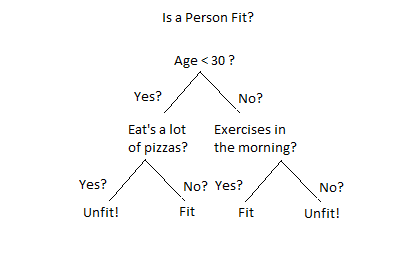
\includegraphics[width=\textwidth]{images/Decision-Trees.png}
  \caption{Decision Tree}
  \label{fig:fullwidth}
\end{figure}
	
	That is a simple example for a decision tree. It is designed to tell whether a person is fit based on its age, its pizza eating behavior and its exercise routine. The root node splits the data into two subsets. One subset contains all people who are under 30 years of age and the other one contains every person who is at least 30 years of age. The subset with the people who are younger than 30 years is split again into subsets of people who are younger than 30 and eat a lot of pizza and into a subset with people who are younger than 30 and don’t eat a lot of pizza. Every person in the subset in which people are younger than 30 and eat a lot of pizza is considered unfit according to the decision tree and every person who is younger than 30 but doesn’t eat a lot of pizza is considered fit. The same practice is applied to the people that are at least 30 years of age and either exercise in the morning and don’t exercise in the morning.\\	
	How are they constructed based on the data? In general, for Boolean features in the data a simple yes or no question if sufficient. If we have continuous values for a feature, we simply split the data using a threshold in the scale of that feature. We ask “is the value smaller than our threshold or is it greater than or equal to our threshold?”. How do we decide what our threshold is? To solve that we follow a simple rule which is supposed to measure the quality of the split. One common rule that is used is the entropy-based information gain. This rule defines that the splits are chosen in a way so that the entropy of the data within the two created subsets is as low as possible. We can understand the entropy in a subset to be low when the class concentration in this subset is high. When 80\% of the data belongs to one class and the other 20\% belong to another class than the entropy is higher as if we have 5 different class belongings that each make up 20\% of the data set. In other words, the splits are chosen so that the emerging subsets are as pure as possible. In practice we define a list of parameters that limit the tree in certain dimensions or its splitting behavior to prevent it from overfitting. We can specify the maximum depth of a tree, the minimum number of samples per leaf and the minimum impurity decrease required to perform a split. In the section hyperparameter tuning we will discover what concrete parameters we tune for our tree-based XGBoost model.\\
	We shortly emphasize the behavior of a decision tree. It “learns” from the data in the moment it is created by recursively splitting the data into subsets that are increasingly pure in terms of their classification. \\
	
	The other concept we need to understand is called random forests.
	
	\subsubsection{Random Forests}
	
	Random forests come from a concept called “ensemble learning”. It is a concept that is based on the fact that more models sometimes can make better predictions than fewer models when aggregated together. We learned before, that decision trees perform classification or regression by recursively asking yes or no questions to the data that split the data into subsets of highest possible purity.
When we apply ensemble learning to decision trees it means that we train multiple trees \cite{55} – hence the name forest – and then combine their predictions by using them as votes for the final prediction. In order to make sense out of that we need to create different trees in the process and we need to make sure that we do not end up with the same tree multiple times since just having the same tree multiple times doesn’t improve our predictions. We can ensure that the trees are all slightly different with altering different parameters for each tree. The technical term for that is uncorrelatedness among the trees. One possibility to ensure uncorrelatedness is called bootstrapping. This is creating smaller data sets out of our original data set. With normal decision trees we feed the whole data set to the tree. However, with bootstrapping we create many slightly different subsets of the data and feed these different subsets to the trees. Being fed different data generally means that the trees are constructed differently. Combining the predictions of many trees that are different because bootstrapping was used is called bootstrap aggregating or for short “Bagging”.\\
Another method we can use to introduce variation to our trees is by shuffling which features a certain tree sees. This concept is called “feature randomness”. While with bootstrapping we divided the data into many different subgroups of smaller size but with the same number of features, feature randomness relies on creating subspaces of features to make the trees behave differently. So, if we have features A, B and C in our data then one tree might only see features A and B while another tree only sees the features B and C.\\
Every tree makes a contribution to the final prediction in form of a vote. In the case of regression, the overall prediction is the average of the predictions of the single trees while in classification the class that was predicted by most trees is the overall prediction. The idea behind it is straight forward. When we use multiple slightly different trees to average their outcome then we can benefit from statistically better and smoother performance. This is due to the fact that the ensembled prediction of those trees over many trials always outperforms the prediction of one single tree that it consists of.

	\subsection{XGBoost}
	
	Ok, after getting to know decision trees and random forests we now look at how exactly an XGBoost model works. Its name is short for extreme gradient boosting. \\
	XGBoost models use a principle called boosting. It works by combining weak learners sequentially to improve the predictive accuracy with each learner \cite{55}. The model starts with one prediction for each data point. For regression tasks that prediction typically just is the mean of all target values. With the first prediction the model computes the errors from every data point to the prediction. After that the first tree is learned. It takes the computed errors as well as the first and second derivative of the loss function and learns splits that group similar errors together. After having the data points grouped by a similar error of the initial prediction, a correction for the initial prediction is computed for each group of data points in the leaf nodes by taking into consideration the first and second derivative of the loss function with the given input. The first derivative tells us simply how strong and in which direction we can reduce our error but it doesn’t tell us how far we can go until we again would worsen the prediction. To help with that, we use the second derivative that tells us how strong the course of the loss function is curved. In other words, it tells us how strong the gradient of the function changes. The extreme in extreme gradient boosting stands for a couple of mechanisms the model uses to make it fast, efficient and accurate. One of these mechanisms is to use the second derivative to compute the adjustment value. Another mechanism which is used is called L2- regularization. It regularizes the weights of leaf nodes by giving penalties for too large values at the leaves preventing the model from overfitting. Other regularizations are used to generalize the model and prevent overfitting for example a maximum tree depth value. After learned, the adjustment values are multiplied with a learning rate that is fix for the whole model and then added to the prediction. This process can repeat a lot of times. Every iteration creates a new tree that again adjusts the predictions of all data points slightly towards the right direction. If the learning rate is lower, one tree adjusts the prediction only slightly so more trees would be needed but they can have a better accuracy since they correct the predictions with a finer granularity. 
	
	
	
	\section{Volatility}
	Because for our stock selection we rely on volatility, we have to define very detailed what we mean by volatility and how we measure it. Volatility is known as the degree to which data disperses over time or in other words “Volatility is a statistical measure of the dispersion of returns for a given security or market index. It is often measured from either the standard deviation or variance between those returns.” – Investopedia - \cite{15}. We understand that the volatility has to be measured to deliver meaningful results. The most common way to measure the volatility of stock courses in finance is by calculating the standard deviation or more precise the sample standard deviation of logarithmic returns \cite{16}. If we do that, we get a measure that tells us how strongly the data points differ on average from the mean of the values. That’s quite good to compare the volatility of different stocks or ETFs. \\
	To do so, we first need to calculate the logarithmic returns. We choose to calculate logarithmic returns instead of simple returns. We can understand why we choose the logarithmic return over the simple return by looking at a simple example.
We calculate the simple return with\\


\begin{equation}
R_i = \frac{P_i - P_{j}}{P_{j}}
\end{equation}

where:\\\\
\begin{tabularx}{\textwidth}{@{}l@{\hspace{2em}--\hspace{2em}}X@{}}
  $R_i$ & simple return of the current data point \\
  $P_i$ & value of the current data point \\
  $P_j$ & value of the previous data point \\
\end{tabularx}\\\\



Let’s say we have a stock price development for some company Xyz of the following: 

\begin{tabularx}{\textwidth}{@{}l*{3}{>{\centering\arraybackslash}X}@{}}
\toprule
            & Month 1 & Month 2 & Month 3 \\
\midrule
Stock price & \$100   & \$150   & \$100   \\
Simple returns & –     & +50.00\% & –33.33\% \\
\bottomrule
\end{tabularx}\\

Since the price ends up at \$100 again, we know that the total return is $0\%$. But when looking at the returns, we have:

\begin{itemize}
  \item Month 1–2: $+50\%$
  \item Month 2–3: $-33.33\%$
\end{itemize}

then we might assume that the average return is:

\[
\frac{-33.33\% + 50\%}{2} = 8.335\%
\]

which is clearly wrong.\\
The mistake here comes from not accounting for compound of interest. The \$50 change from Month 2 to Month 3 is based on a value of \$150. The change from Month 1 to Month 2 is based on \$100. 

Although both changes are \$50, the relative change is different. To correctly calculate the total return, we must multiply the returns rather than averaging them:

\[
150\% \times 66.7\% = 100\%
\]

This gives us a final value equal to our starting value, i.e., a total return of $0\%$. This is where using log returns becomes more intuitive when looking at returns over time steps. Let’s extend our course of the stock price by another 4 months:\\

\begin{tabularx}{\textwidth}{@{}l*{7}{>{\centering\arraybackslash}X}@{}}
\toprule
             & Month 1 & Month 2 & Month 3 & Month 4 & Month 5 & Month 6 & Month 7 \\
\midrule
Price        & \$100   & \$150   & \$100   & \$150   & \$100   & \$150   & \$100   \\
Simple Return & –      & +50.00\% & –33.33\% & +50.00\% & –33.33\% & +50.00\% & –33.33\% \\
\bottomrule
\end{tabularx}\\


If we look at returns like these, we could easily think that we end up with a positive return overall but when looking at the actual stock price we see, that we are just oscillating between two values. When we use the logarithmic returns, it gets more intuitive. We calculate the logarithmic return using: \cite{17}\\


\begin{equation}
  R_i = \ln\left( \frac{C_i}{C_{i-1}} \right)
\end{equation}
\medskip
where..:\\
\begin{tabularx}{\textwidth}{@{}l@{\hspace{2em}--\hspace{2em}}X@{}}
  $R_i$      & logarithmic return at the current data point \\
  $\ln$      & natural logarithm \\
  $C_i$      & current data point’s value \\
  $C_{i-1}$  & previous data point’s value \\
\end{tabularx}\\

\begin{minipage}{\textwidth}
We calculate the logarithmic return for our stock course.\\
\begin{tabularx}{\textwidth}{@{}l*{7}{>{\centering\arraybackslash}X}@{}}
\toprule
             & Month 1 & Month 2 & Month 3 & Month 4 & Month 5 & Month 6 & Month 7 \\
\midrule
Price        & \$100   & \$150   & \$100   & \$150   & \$100   & \$150   & \$100   \\
Simple Return & --     & +50.00\% & -33.33\% & +50.00\% & -33.33\% & +50.00\% & -33.33\% \\
$\ln$ Return & --     & 0.405   & -0.405  & 0.405   & -0.405  & 0.405   & -0.405  \\
\bottomrule
\end{tabularx}\\
\end{minipage}\\


If we add up the logarithmic returns, we are left with $3 \times (0.405) - 3 \times (0.405)$ which is 0. So, using the logarithmic return instead of actual stock prices itself or simple returns of the stock prices, leaves us with numbers that are detached from the constantly altering scale of stock prices. We now have our logarithmic returns, which leads us to the next step which is calculating the volatility based on them.\\

The most common way to calculate the volatility is by calculating the sample standard deviation. We use the following formula.\\

\begin{equation}
s = \sqrt{\frac{1}{n - 1} \sum_{i=1}^{n} (x_i - \bar{x})^2}
\end{equation}
where..:\\
\begin{tabularx}{\textwidth}{@{}l@{\hspace{2em}--\hspace{2em}}X@{}}
  $n$      & number of data points the sample standard deviation is calculated for \\
  $x_i$    & the current data point at $i$ (here: the logarithmic return at time $i$) \\
  $\bar{x}$ & the mean of all data points (here: the mean of all logarithmic returns) \\
\end{tabularx}\\\\

In our codebase we write our own pipeline to calculate the volatility in the way we just discussed. For that we use a pre-implemented function for the sample standard deviation which is located in pandas.DataFrame.std(). The standard deviation gives information about how strongly the data points are deviated from the statistical mean. If the standard deviation is lower it means that the data points are on average closer to the mean and if the standard deviation is higher, it means that the data points are spread wider.\\\\
We defined a measure that tells us how volatile assets have been in the past. The volatility score is averaged over our time frame which is about 5 years. We could go ahead and select the stocks based on that score. If we do so, we might see, that stocks with the same volatility score seem to still have much different characteristics in the data. \\
To understand that we look at two hypothetical stocks. One stock is oscillating moderately strong throughout the whole course let’s say its volatility score is 5 at every point in time. The other stock oscillates compared to the first one very little during the first half but much more during the second half. Let’s say during the first half it has a volatility score of 1 and during the second half it has a volatility score of 9. The average volatility of these two stocks over the whole course is 5 even though they have very different characteristics and the first stock has a more constant oscillation which doesn’t change as much with time. To account for that problem and to make sure that the stocks we choose are as similar as possible in terms of their volatility we look at another metric which is the volatility of the volatility. As one might think, this metric simply measures how much the volatility changes over time. To measure that, we calculate the pure volatility, just as described above, not for the whole set of data but instead multiple times for rolling windows. So, we basically compute the volatility for every sequence 75 consecutive data points in the data set. After having the volatility for each of these windows we again calculate, just as explained above, the volatility of these volatility measures. Like that we get the volatility of the volatility for our assets or in other words we get a measurement for how constant a volatility is for one asset or how strong it changes over time.\\\\

Having these metrics available we can now choose the stocks or ETFs and retrieve their historical data to train our models.


	\section{Stock Selection}
	We have defined how we measure the volatility of a stock course. That enables us now to choose stock data based on which we want to train our models. We are using the alpaca-trade-api to retrieve our historical stock data. After we created ourself an account and retrieved the credentials, we now create a list which contains common stocks and ETFs listed on AMEX, ARCA, BATS, NYSE, NASDAQ or NYSEARCA \cite{18}. After that we define the time frame for which we want to retrieve the historical data, we choose it to be the past 5 years. Like that we retrieve the historical prices of about 11500 stocks and ETFs. \\
	We further process this data to be only left with a table with the stock symbols as columns, the timestamp as index and the close price as a column as well. During preprocessing we would need to account for missing values. It would be much easier to already now just choose the stocks and ETFs without missing values. We look how many of the stocks and ETFs are having missing values in their data and its about 5000. That means we have about 6500 stocks and ETFs left with no missing values. Since we only need a handful of historical courses, we simply decide to drop all that have missing values and just proceed with the ones without any missing value. Besides that, we also drop all historical courses that have the same closing price over at least 30 days. When a stock or ETF has the same closing price over a number of days it can have different reasons but it usually means that the asset hasn’t been traded during that time. If the price stays the same for a longer period, we don’t want the assets course in our data because it is obviously not natural behavior of the market and anomalies of this kind make it harder for the algorithm to learn. \\\\
	
	We want to extract information regarding volatility. To do so we apply the methods of calculating the volatility and calculating the volatility of the volatility for our assets as described in the previous section. We apply the functions and store the returned values in a table. As we understood before we want the volatility of the volatility to be as low as possible for all stock and ETF courses while at the same time having a wide range of different volatilities of which we choose stocks and ETFs to train our model. To filter out stocks and ETFs that have a higher volatility of volatility we need to visualize our data set. For that we draw a graph. The graph shows the measure of volatility (blue) and volatility of volatility (orange) on the y-axis for each stock or ETF and the number of the stocks on the x-axis. We sort the stocks by the volatility of their volatility in increasing order.\\
	
\begin{figure}[htbp]
  \centering
  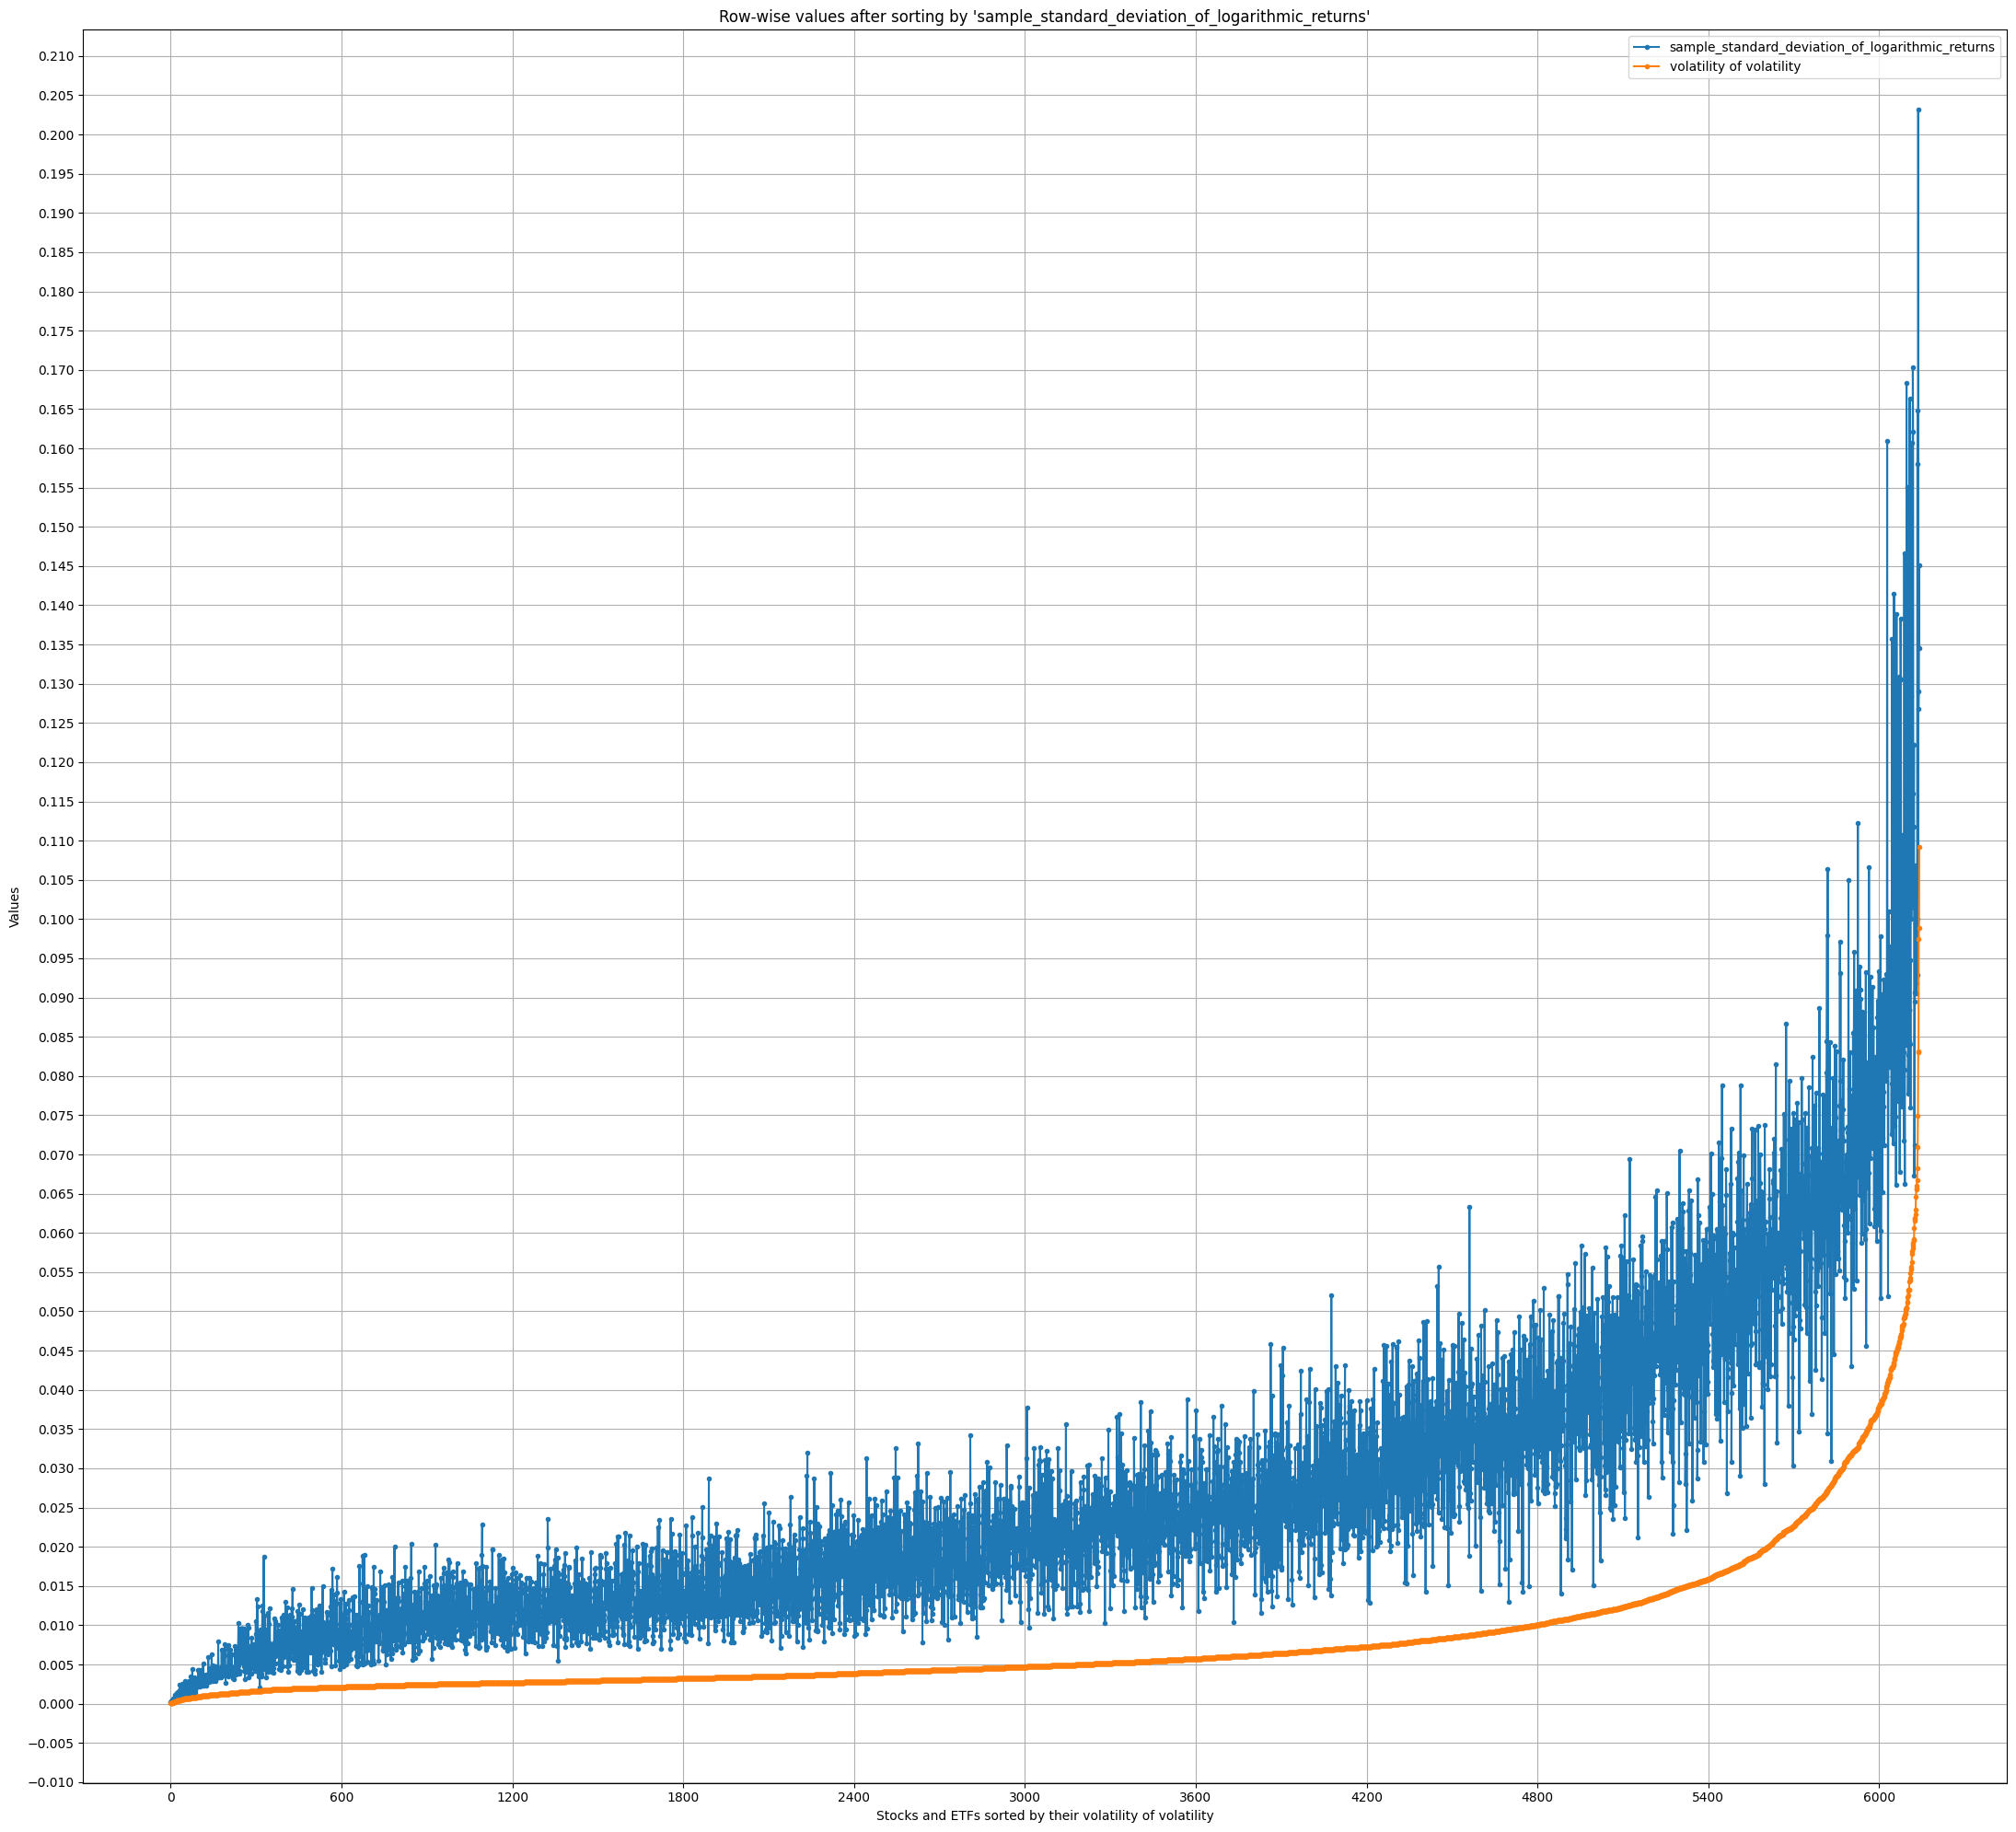
\includegraphics[width=\textwidth]{images/vol_of_vol.png}
  \caption{Assets sorted by volatility of their volatility}
  \label{fig:fullwidth}
\end{figure}
	
	We see that the volatility of the volatility seems to correlate on average with the volatility. The greater the volatility of the volatility the greater the pure volatility. Now, for us two things are most important. The first is, we want to have stocks from volatilities within a range that is as wide as possible to have a more meaningful result of our experiment. The second is, we want the volatility of the volatility to be as low as possible. We explained before why we want that. That means we need to look for a threshold at which we cut off the data. Since the volatility seems to correlate with the volatility of the volatility, we need to make a compromise when deciding for a threshold. We will drop every stock or ETF that has a volatility of volatility greater than that. We take into consideration that we only need a relatively small number of stocks and ETFs per bin, about 15. Besides that, we take into consideration that the volatility of volatility seems to increase dramatically on the right side of the graph so we definitely want to cut off at some point before it’s dramatic increase. After careful consideration we decide to cut off all stocks and ETFs that have a volatility of their volatility of more than 0.01. This is pretty much at stock 4800 in the graph. Like that we ensure to have constant oscillation based on the given volatility while still being able to capture a wide range of stocks and ETFs with different volatilities. \\
	Across the range of volatility, we want to evenly pick 5 values for each of which we again pick 15 stocks or ETFs that are as close as possible to the values in terms of volatility of the historical data. To get a sense for that we first construct bins of volatility and sort our stocks and ETFs into these bins. We plot the distribution of all assets and how they fit into steps of volatility.\\
		
\begin{figure}[htbp]
  \centering
  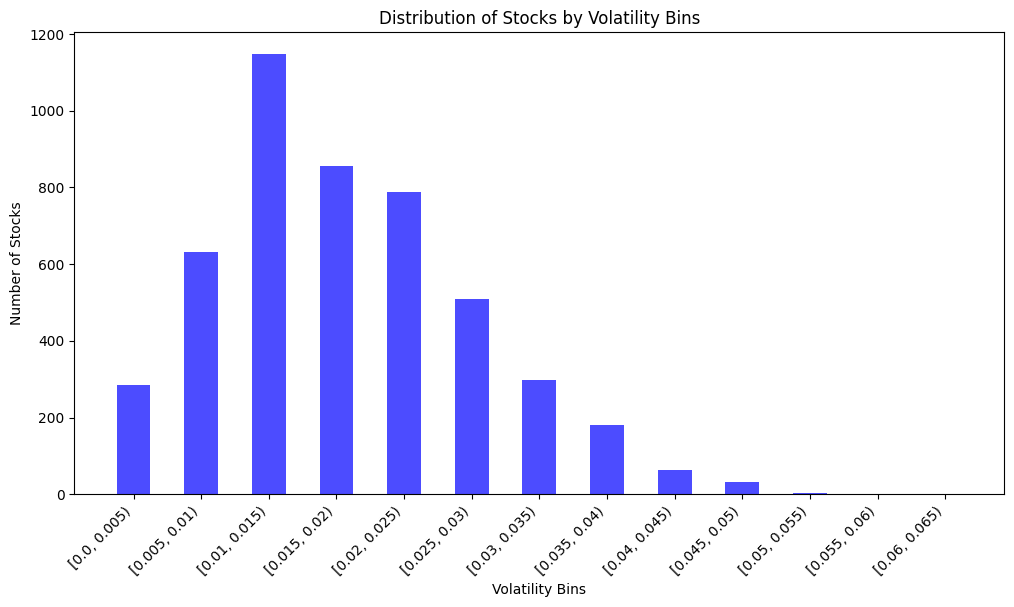
\includegraphics[width=\textwidth]{images/bins.png}
  \caption{Distribution of assets according to volatility intervals}
  \label{fig:fullwidth}
\end{figure}


We now want to manually choose 5 bins and 15 stocks or ETFs for each bin for training. To make the results as meaningful as possible we define the ranges of our bins in a way so that we capture the widest possible range of volatility. In other words, we want bin1 and bin5 to be as far apart as possible on the graph and the remaining 3 bins to be in between them while having equal distances to their neighbors. At the same time, we want the stocks and ETFs within one bin to be as similar as possible in terms of their volatility. Based on the distribution which is visible in the plot, we choose five volatility bins to be:


\textbf{\begin{table}[h!]
\centering
\renewcommand{\arraystretch}{1.4}
\begin{tabularx}{0.4\textwidth}{@{}>{\centering\arraybackslash}X@{}}
\toprule
\textbf{Volatility bins} \\
\midrule
1. 0.00235 -- 0.00270 \\
2. 0.01243 -- 0.01248 \\
3. 0.02243 -- 0.02250 \\
4. 0.03242 -- 0.03260 \\
5. 0.04500 -- 0.04600 \\
\bottomrule
\end{tabularx}
\end{table}
}





\begin{figure}[htbp]
  \centering
  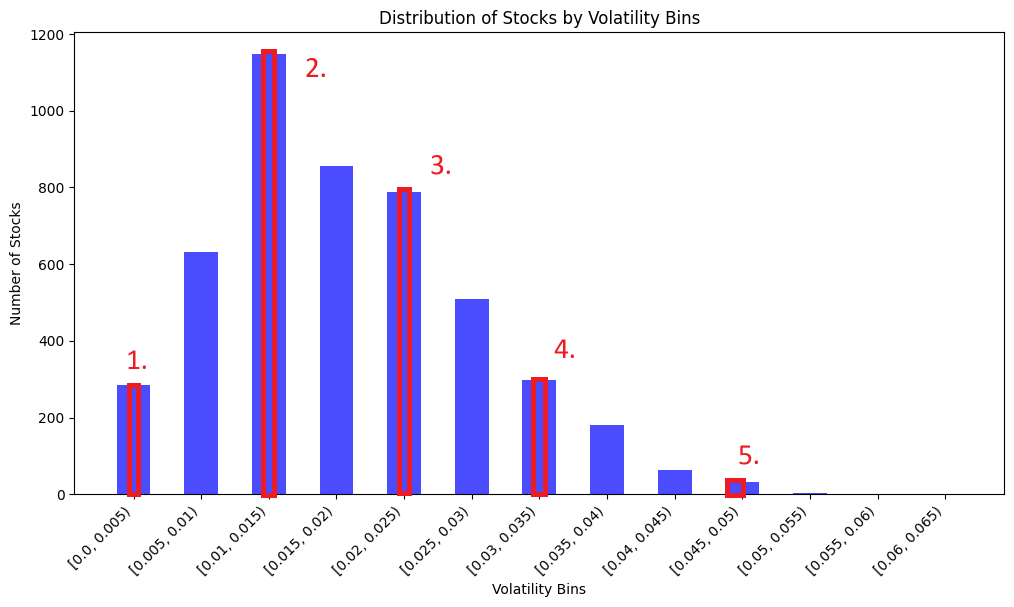
\includegraphics[width=\textwidth]{images/volatility_bins.png}
  \caption{approximate selected ranges for 5 bins}
  \label{fig:fullwidth}
\end{figure}
	
	
	This will allow us to train and evaluate the models based on multiple stock data for each value of volatility which we expect to give us a statistically better and closer to the average measurement compared to just using one stock for each step which is susceptible to outliers and noise. We especially expect the models to have a similar predictive accuracy for stocks within the same volatility interval and to show clear jumps in performance when trained based on stocks of different intervals. 
	
	\section{Data Preprocessing}
	
During the previous section we selected the stocks that can be grouped into 5 intervals or bins of different volatility and which we want our models to be evaluated on. Since we already dropped stocks with missing values, we don't need to perform any further imputation. Our historical data so far has the features: open, high, close, low, vwap, volume, trade\_count, symbol – where symbol is the ticker symbol of the stock and will not be used for training.\\
The other features are:


\begin{itemize}
  \item \textbf{trade\_count} --- which tells how many transactions have been made in a period.
  \item \textbf{Volume} --- which is the number of shares that have been traded within a period.
  \item \textbf{Volume Weighted Average Price (VWAP)} --- which is the typical price of a stock or ETF weighted by its volume \cite{36}.
  \item \textbf{Open} --- the price at which the first trade occurred during the period.
  \item \textbf{Close} --- the price at which the last trade occurred during the period.
  \item \textbf{High} --- the highest traded price during the period.
  \item \textbf{Low} --- the lowest traded price during the period.
\end{itemize}

\vspace{1em}
\begin{minipage}{\textwidth}

The VWAP is calculated as:

\begin{equation}
\mathrm{VWAP} = \frac{\sum_{i=1}^n P_i \cdot V_i}{\sum_{i=1}^n V_i}
\end{equation}
\end{minipage}

where..:\\

\begin{tabularx}{\textwidth}{@{}l@{\hspace{2em}--\hspace{2em}}X@{}}
  $P_i$ & the price of the trade $i$ \\
  $V_i$ & the volume of the trade $i$ \\
  $n$   & the total number of trades in the period \\
\end{tabularx}

	So, if within one period particularly many trades are executed at a certain price than this price is weighted more than a price at which fewer trades were executed. That means while the close only tells you the price at which the last trade executed, VWAP is averaged over all trades in that day.\\\\
	
	The next step is to preprocess the historical data from each asset by adding other features. Some of those are retrieved from APIs and some are calculated using the existing features. We choose the features based on those, the review study by Kumbure et al. \cite{5} has shown to be mainly used in stock price forecasting. We also add some indicators mentioned in the articles “Template:Technical analysis” from Wikipedia \cite{20} and “Technical Indicator: Definition, Analyst Uses, Types and Examples” from Investopedia \cite{21}. 
	
		\subsection{Feature Engineering}
		
			\subsubsection{Relative Strength Index (RSI)}
			
The RSI is a way to measure speed and directions of price movements. The RSI always lies in the range of zero to 100 and it is commonly considered overbought when above 70 and oversold when below 30. It is a measure that carries a value for every period and is calculated as:\\


\begin{equation}
\mathrm{RSI} = 100 - \frac{100}{1 + RS}
\end{equation}

where

\[
RS = \frac{\text{Average Gain over } n \text{ periods}}{\text{Average Loss over } n \text{ periods}}
\]

and\\

\begin{tabularx}{\textwidth}{@{}l@{\hspace{2em}--\hspace{2em}}X@{}}
  $n$ & number of periods (typically 14) \\
  Average Gain & average of all absolute gains over the last $n$ periods \\
  Average Loss & average of all absolute losses over the last $n$ periods \\
\end{tabularx}\\
			
Where Average Gain and Average Loss are Exponentially weighted moving averages \cite{22}. Exponentially weighted moving averages are averages that weigh the recent component more than previous components. 
			
			\subsubsection{Rate of Change (ROC)}
			The ROC is an indicator that shows the return in percent compared to the price n periods ago. A common number for n is 14. \cite{23}
			
\begin{equation}
\text{ROC}_t = \frac{P_t - P_{t-n}}{P_{t-n}} \times 100\%
\end{equation}
where..:\\

\begin{tabularx}{\textwidth}{@{}l@{\hspace{2em}--\hspace{2em}}X@{}}
  $P_t$     & is the price at the current period $t$ \\
  $P_{t-n}$ & is the price $n$ periods ago \\
  $n$       & is the number of periods over which the change is calculated \\
\end{tabularx}

			
			\subsubsection{Moving Average Convergence Divergence (MACD)}
			The MACD is used to measure both the momentum and direction of a price movement. It consists of a the MACD line and the signal line. The MACD line measures the difference between a shorter exponential moving average and a longer exponential moving average. The signal line is again an exponential moving average of the MACD line. Due to the fact that both lines crossing has implications for the price movement and we want the model to better identify that relation, we also add a histogram feature that simply is calculated as the difference between MACD line and signal line. \cite{24}\\
			
\begin{equation}
\text{MACD}(t) = \text{EMA}_{\text{short}}(t) - \text{EMA}_{\text{long}}(t)
\end{equation}

\begin{equation}
\text{Signal}(t) = \text{EMA}_{\text{signal period}} \big(\text{MACD}(t)\big)
\end{equation}

\begin{equation}
\text{Histogram}(t) = \text{MACD}(t) - \text{Signal}(t)
\end{equation}

where..:\\

\begin{tabularx}{\textwidth}{@{}l@{\hspace{2em}--\hspace{2em}}X@{}}
  $\text{EMA}_{\text{short}}$       & is the exponential moving average over a short period (e.g., 12 days) \\
  $\text{EMA}_{\text{long}}$        & is the exponential moving average over a long period (e.g., 26 days) \\
  $\text{EMA}_{\text{signal period}}$ & is the exponential moving average of the MACD line over the signal period (e.g., 9 days) \\
  $\text{MACD}(t)$                  & is the MACD value at time $t$ \\
  $\text{Signal}(t)$                & is the Signal line value at time $t$ \\
  $\text{Histogram}(t)$             & is the Difference between MACD and Signal line at time $t$ \\
\end{tabularx}

			\subsubsection{Stochastic Oscillator}
			
The stochastic Oscillator is another momentum indicator that measures where the current closing price lies in the range of the highest high of a certain past period and the lowest low of that same period in percent. This value is called \%K. A second value which is called \%D contains the moving average of \%K for a short period. Since again the relation of those two lines is of importance to us and we need to make the machine learning model aware of it, we add a stochastic difference value that is calculated as the difference of these 2 values. \cite{25}\\

\begin{equation}
\begin{aligned}
  \%K(t) &= 100 \times \frac{P(t) - L_n(t)}{H_n(t) - L_n(t)}  \\
  \%D(t) &= \text{SMA}_m(\%K(t))\\
  \text{StochDiff}(t) &= \%K(t) - \%D(t)\\
\end{aligned}
\end{equation}

\begin{minipage}{\textwidth}

where..:\\

\begin{tabularx}{\textwidth}{@{}l@{\hspace{2em}--\hspace{2em}}X@{}}
  $P(t)$         & is the current closing price at time $t$ \\
  $H_n(t)$       & is the highest price over the last $n$ periods up to time $t$ \\
  $L_n(t)$       & is the lowest price over the last $n$ periods up to time $t$ \\
  $\%K(t)$       & is the fast stochastic oscillator value at time $t$ \\
  $\%D(t)$       & is the moving average (usually simple) of $\%K(t)$ over $m$ periods \\
  $\text{SMA}_m$ & is the simple moving average over $m$ periods \\
  $\text{StochDiff}(t)$ & is the difference between $\%K(t)$ and $\%D(t)$ at time $t$ \\
\end{tabularx}

\end{minipage}

			\subsubsection{Commodity Channel Index (CCI)}

The CCI measures how far a price is from its statistical average indicating overbought or oversold market conditions. \cite{26}\\

\begin{equation}
\begin{aligned}
  TP(t) &= \frac{H(t) + L(t) + C(t)}{3} \\\\
  SMA_{TP}(t) &= \frac{1}{n} \sum_{i=0}^{n-1} TP(t-i) \\\\
  MAD(t) &= \frac{1}{n} \sum_{i=0}^{n-1} |TP(t-i) - SMA_{TP}(t)| \\\\
  CCI(t) &= \frac{TP(t) - SMA_{TP}(t)}{0.015 \times MAD(t)} \\\\
\end{aligned}
\end{equation}


\begin{minipage}{\textwidth}

where..:\\

\begin{tabularx}{\textwidth}{@{}l@{\hspace{2em}--\hspace{2em}}X@{}}
  $H(t)$         & is the highest price at time $t$ \\
  $L(t)$         & is the lowest price at time $t$ \\
  $C(t)$         & is the closing price at time $t$ \\
  $TP(t)$        & is the typical price at time $t$ \\
  $SMA_{TP}(t)$  & is the simple moving average of typical prices over $n$ periods at time $t$ \\
  $MAD(t)$       & is the mean absolute deviation of typical prices over $n$ periods at time $t$ \\
  $CCI(t)$       & is the Commodity Channel Index at time $t$ \\
  $n$            & is the number of periods used for SMA and MAD calculations \\
  $0.015$        & is a constant to ensure that approximately 70-80\% of CCI values fall between -100 and +100 \\
\end{tabularx}

\end{minipage}

			\subsubsection{Moving Averages}
			We add multiple simple moving averages with different window sizes. Moving averages smooth out price data and indicate an upwards trend when increasing and a downwards trend when decreasing. Besides that, they can indicate overbought or oversold conditions \cite{27}. \\
			
			
\begin{equation}
\begin{aligned}
  \text{SMA}_n(t) &= \frac{1}{n} \sum_{i=0}^{n-1} P(t - i)
\end{aligned}
\end{equation}

\begin{minipage}{\textwidth}

where..:\\

\begin{tabularx}{\textwidth}{@{}l@{\hspace{2em}--\hspace{2em}}X@{}}
  $P(t)$ & is the price (e.g. closing price) at time $t$ \\
  $n$    & is the number of periods used in the moving average \\
\end{tabularx}
\end{minipage}

			\subsubsection{Average True Range (ATR)}
			
			The ATR is a volatility indicator that tells how much the price moves on average per period. We therefore first look at the True Range (TR) for every period. This is the maximum price difference within that period. We add that difference to our feature set. We use the previous day’s close price because the current day’s open price can differ from the previous day’s close price due to overnight news and market shift \cite{30}. After that we use wilder’s smoothing to smooth out the True Range over a certain windows size, usually 14, so that we understand how volatile certain periods are \cite{31}. 
			
			
\begin{equation}
\begin{aligned}
  \text{TR}(t) &= \max \big( H(t) - L(t), |H(t) - C(t-1)|, |L(t) - C(t-1)| \big) \\
  \text{ATR}_n(t) &= \frac{1}{n} \sum_{i=0}^{n-1} \text{TR}(t - i)\\
  \text{ATR}_n(t) &= \frac{(\text{ATR}_n(t-1) \times (n - 1)) + \text{TR}(t)}{n}\\
\end{aligned}
\end{equation}


\begin{minipage}{\textwidth}

where..:\\

\begin{tabularx}{\textwidth}{@{}l@{\hspace{2em}--\hspace{2em}}X@{}}
  $H(t)$       & is the highest price at time $t$ \\
  $L(t)$       & is the lowest price at time $t$ \\
  $C(t)$       & is the closing price at time $t$ \\
  $\text{TR}(t)$ & is the true range at time $t$, defined as the maximum of: the current high minus low, the absolute difference between current high and previous close, and the absolute difference between current low and previous close \\
  $n$          & is the number of periods over which the ATR is calculated \\
  $\text{ATR}_n(t)$ & is the average true range at time $t$, computed as the simple average of the true range over the last $n$ periods \\
\end{tabularx}
\end{minipage}

			
			
			
			\subsubsection{Average Directional Index (ADX)}
			The ADI uses the ATR as a component. The ADI and its components measure how much of the Average movement within a certain window which we derive from the ATR is upwards movement and how much is downwards movement. We calculate the up and downwards movement like this \cite{32}. +DM now stores all absolute increases in the high value for periods in which the low value decreased less than the high value increased. -DM works vice versa. We now average these two values over a window that must have the same size as the window size n from our ATR. Like that we get the average up and down movement in absolute values for the given window. We derive the overall movement from the ATR and calculate the percent to which it is upwards movement or downwards movement. The next step lets us calculate the Directional Movement Index (DX). DX tells us in percent how one-sided a movement is. If up and down movement have the same portion of the overall movement then DX is 0%. If DX is positive then upwards movements have a greater proportion of the overall movement. The last step is to calculate the actual ADX. We again use wilder’s smoothing. That is a recursive function so we need to calculate the first ADX value manually by simply averaging the previous n DX values. Any further ADX value is calculated recursively.\\
			
\begin{equation}
\begin{aligned}
  \text{+DM}(t) &= 
    \begin{cases} 
      H(t) - H(t-1) & \text{if } H(t) - H(t-1) > L(t-1) - L(t) \text{ and } H(t) - H(t-1) > 0 \\
      0 & \text{otherwise}
    \end{cases}
    \quad & \text{(positive directional movement)} \\
  \text{-DM}(t) &= 
    \begin{cases} 
      L(t-1) - L(t) & \text{if } L(t-1) - L(t) > H(t) - H(t-1) \text{ and } L(t-1) - L(t) > 0 \\
      0 & \text{otherwise}
    \end{cases}
    \quad & \text{(negative directional movement)} \\
  \text{TR}(t) &= \max \big( H(t) - L(t), |H(t) - C(t-1)|, |L(t) - C(t-1)| \big) \quad & \text{(true range)} \\
  \text{+DI}_n(t) &= 100 \times \frac{\text{Smoothed } +DM_n(t)}{\text{ATR}_n(t)} \quad & \text{(positive directional index)} \\
  \text{-DI}_n(t) &= 100 \times \frac{\text{Smoothed } -DM_n(t)}{\text{ATR}_n(t)} \quad & \text{(negative directional index)} \\
  \text{DX}(t) &= 100 \times \frac{|\text{+DI}_n(t) - \text{-DI}_n(t)|}{\text{+DI}_n(t) + \text{-DI}_n(t)} \quad & \text{(directional movement index)} \\
  \text{ADX}_n(t) &= \frac{1}{n} \sum_{i=0}^{n-1} \text{DX}(t - i) \quad & \text{(average directional index, initial)} \\
  \\
  \text{ADX}_n(t) &= \frac{(\text{ADX}_n(t-1) \times (n - 1)) + \text{DX}(t)}{n} \quad & \text{(recursive smoothing)} \\
\end{aligned}
\end{equation}



\begin{minipage}{\textwidth}

where..:\\

\begin{tabularx}{\textwidth}{@{}l@{\hspace{2em}--\hspace{2em}}X@{}}
  $H(t)$           & is the highest price at time $t$ \\
  $L(t)$           & is the lowest price at time $t$ \\
  $C(t)$           & is the closing price at time $t$ \\
  $\text{+DM}(t)$  & is the positive directional movement at time $t$ \\
  $\text{-DM}(t)$  & is the negative directional movement at time $t$ \\
  $\text{TR}(t)$   & is the true range at time $t$ (see ATR formula) \\
  $\text{ATR}_n(t)$ & is the average true range over $n$ periods \\
  $\text{+DI}_n(t)$ & is the positive directional index over $n$ periods \\
  $\text{-DI}_n(t)$ & is the negative directional index over $n$ periods \\
  $\text{DX}(t)$   & is the directional movement index at time $t$ \\
  $\text{ADX}_n(t)$ & is the average directional index over $n$ periods, indicating trend strength \\
  $n$              & is the number of periods used for smoothing and calculation \\
  \text{Smoothed } & refers to applying Wilder’s smoothing\\
\end{tabularx}
\end{minipage}

			\subsubsection{Bollinger Bands}
			The Bollinger Bands are indicators to gauge the volatility of a stock to understand whether they are over or undervalued \cite{33}. Since we use this indicator for machine learning purposes, we will add the following features to emphasize relations among the bands or between our close price and the bands.\\
\begin{equation}
\begin{aligned}
  \text{MiddleBand}_n(t) &= \frac{1}{n} \sum_{i=0}^{n-1} C(t - i)\\
  \text{StdDev}_n(t) &= \sqrt{\frac{1}{n} \sum_{i=0}^{n-1} \big(C(t - i) - \text{MiddleBand}_n(t)\big)^2}\\
  \text{UpperBand}_n(t) &= \text{MiddleBand}_n(t) + k \times \text{StdDev}_n(t) \\
  \text{LowerBand}_n(t) &= \text{MiddleBand}_n(t) - k \times \text{StdDev}_n(t)  \\
  \\
  \%B(t) &= \frac{C(t) - \text{LowerBand}_n(t)}{\text{UpperBand}_n(t) - \text{LowerBand}_n(t)}\\
  \text{Bandwidth}_n(t) &= \frac{\text{UpperBand}_n(t) - \text{LowerBand}_n(t)}{\text{MiddleBand}_n(t)}\\
  \\
  \text{DistToUpper}_n(t) &= \text{UpperBand}_n(t) - C(t)\\
  \text{DistToLower}_n(t) &= C(t) - \text{LowerBand}_n(t)\\
\end{aligned}
\end{equation}
where..:\\

\begin{tabularx}{\textwidth}{@{}l@{\hspace{2em}--\hspace{2em}}X@{}}
  $C(t)$                 & is the closing price at time $t$ \\
  $n$                    & is the number of periods used for calculation\\
  $k$                    & is the number of standard deviations for the bands \\
\end{tabularx}

	
			\subsubsection{On-Balance Volume (OBV)}
			The On-Balance Volume Indicator is a momentum indicator that uses volume flow to predict price movement. It assumes that volume precedes the price – so a rising OBV signals buying pressure and a falling OBV signals selling pressure \cite{34}. Besides the absolute OBV we add a normalized OBV for better machine learning suitability and an OBV momentum that compares the OBV to the OBV n periods before. \\
			
\begin{equation}
\begin{aligned}
  \text{OBV}(t) &= 
    \begin{cases}
      \text{OBV}(t-1) + V(t) & \text{if } C(t) > C(t-1) \\
      \text{OBV}(t-1) - V(t) & \text{if } C(t) < C(t-1) \\
      \text{OBV}(t-1)         & \text{otherwise}
    \end{cases}
    \\
  \text{OBV}(t_0) &= 0 
\end{aligned}
\end{equation}
where..:\\

\begin{tabularx}{\textwidth}{@{}l@{\hspace{2em}--\hspace{2em}}X@{}}
  $C(t)$           & is the closing price at time $t$ \\
  $V(t)$           & is the trading volume at time $t$ \\
\end{tabularx}

			
			\subsubsection{Volume Price Trend (VPT)}
			The VPT is a momentum indicator that combines the price change with volume. Its purpose is to track how strongly volume aligns with or contradicts price changes \cite{35}. For Machine Learning purposes we also add the VPT in a normalized way and the VPT momentum.\\
			
\begin{equation}
\begin{aligned}
  \text{VPT}(t) &= \text{VPT}(t-1)
    + V(t)\,\frac{C(t) - C(t-1)}{C(t-1)}
    \\
  \text{VPT}(t_0) &= 0    
\end{aligned}
\end{equation}

\begin{tabularx}{\textwidth}{@{}l@{\hspace{2em}--\hspace{2em}}X@{}}
  $C(t)$            & is the closing price at time $t$ \\
  $V(t)$            & is the trading volume at time $t$ \\
\end{tabularx}\\





			
		\subsection{Macro-economic features}
		We add Macro-economic features to capture global or US wide circumstances and market context \cite{38}. We use the “FRED API” version 0.5.2 to retrieve them \cite{37}. Some of the indicators are not published daily. For example, the GDP is published quarterly. We therefore use the interpolate function that comes with the pandas library. It looks for brackets of NaN values and draws a line from the valid value before and the valid value after the bracket to fill the rows in between linearly. So, if we have a list such as [10, NaN, NaN, NaN, 18, NaN, 26] then the interpolation of this list would return this list: [10, 12, 14, 16, 18, 22, 26]. This allows us to simulate a realistic and smooth course of the features.
			\subsubsection{S\&P 500}
			One important macro-economic indicator is the S\&P 500 index. Since it includes the biggest 500 US companies it is an important measure of the health of the overall us economy.
			\subsubsection{GDP (USA)}
			The Gross domestic Product is the value of all goods and services produced by a country in a given period. It is a meaningful indicator since it reflects the economic performance of a country \cite{38}.
			\subsubsection{unemployment rate}
			The unemployment rate can capture strengths and weaknesses in the economy. It is a great indicator for economic activity \cite{38}.
			\subsubsection{Consumer price index (CPI)}
			The consumer price index measures the monthly change in prices paid by urban US customers for different basic products and services \cite{39}.
			\subsubsection{Personal consumption expenditures (PCE)}
			The personal consumption expenditures is an indicator that measures how much US households spend on goods and services \cite{41}.
			\subsubsection{Industrial Production index (IPI)}
			The industrial production index measures the output in manufacturing, gas, oil, mining and electric industries \cite{42}.
			\subsubsection{federal funds rate}
			The federal funds rate is the target interest rate range at which commercial banks are supposed to borrow money \cite{43}.
			\subsubsection{10Y treasury rate}
			The 10-year treasury is the interest rate which the US government pays to borrow money over a decade. It is an important benchmark for other interest rates and it talks about expectations of the US government about inflation and economic growth \cite{44}.
			\subsubsection{Retail sales}
			Retail sales is a main indicator for economic health because it provides information about the buying power of consumers. Bigger retail sales usually lead to more profit for companies which has a positive effect on the stock price \cite{40}. 
			\subsubsection{housing starts}
			Housing starts is the number of newly started construction projects in a given period that provides information about the housing market and general economic activity \cite{45}. 
			\subsubsection{exchange rates}
Exchange rates are a good way to measure the economic health in comparison to economies from other countries \cite{46} \cite{47}. We include the exchange rates USD-EUR, USD-GBP and USD-JPY.
			\subsubsection{Calendar features}
We also add the following calendar features to capture patterns for example the Monday effect \cite{28} and the January effect \cite{29}.

\begin{itemize}
  \item Day of week (1--7)
  \item Day of year (1--365)
  \item Month (1--12)
  \item Year (yyyy)
  \item Quarter (1--4)
\end{itemize}


In total we now have included 60 features in our data set that are products or byproducts of our calculations. We also add a ‘target’ column with the next days close price which will be our target value during training. We perform further preprocessing steps, but we have to perform them in separate pipelines since the LSTM and the CNN model need distinct preprocessing steps compared to an XGBoost model. 


		\subsection{Connection pipeline for LSTM and CNN preprocessing}
One important step we need to perform on data for neural networks is normalization. This is due to the nature of neural networks – they are sensitive to the scale of input features. Without normalization features with large values would dominate features with small values which would lead to uneven learning. We look at an example to understand that dynamic. Neural networks as we learned before work by taking vectorized inputs. That means they take a list of numerical values as input. Each of these values is multiplied by the according weight and then typically added together. \\

\begin{minipage}{\textwidth}
Let’s say we have the following equation for one neuron and we assume that features x1 and x2 are equally important to the result. We define the value inside the neuron before activation as:\\
We define a linear function as:

\[
y = w_1 x_1 + w_2 x_2 + b
\]

Suppose:

\begin{tabularx}{\textwidth}{@{}l@{\hspace{2em}}X@{}}
  $x_1 = 200$ & (e.g., size in m$^2$) \\
  $x_2 = 3$   & (e.g., number of bedrooms) \\
  $w_1 = 1$   & \\
  $w_2 = 1$   & \\
\end{tabularx}

Then:

\[
y = 1\times200 + 1\times3 + b = 203+b
\]
\end{minipage}\\\\

As we can see, the contribution of x1 to the result is much larger even though we know that both features are equally important, it’s just that x1 has a larger scale. One might argue that the network could compensate this larger scale by using a much smaller weight for input feature x1, but then we are interfering with the nature of the neural network which really is to weigh particular features heavier because they have been observed to have a greater impact on the result. This is not the case for us because we assume that our features both have an equal importance to the result. If we already have different scales for our inputs at the beginning of the network, it would be as if we predefine an importance for each feature. In case we know that particular features are in fact more important than others and we know the size of this importance among the features, than the practice to weigh the more impactful ones heavier would make sense, but that’s not common practice. Now it is totally true that you could simply have much smaller weights for those much larger inputs. But the problem with that lies in the nature of how the network learns its weights. They are computed based on a fixed learning rate which is an absolute value for the whole network and for the full training process. The learning rate tells us how much a weight is updated. If the learning rate is very small it means that we can converge our weights to very precise values with a fine granularity but it also means that we need more iterations to get to this correct value because we are doing much smaller steps. So, if the weights are forced to lie within different ranges because our input features have different scales, then the learning process within the whole network would be asymmetrical and some weights would learn very slow and barely reach a good value while others constantly overshoot and never converge to an accurate enough number. In short this is why normalization is necessary. \\


\begin{minipage}{\textwidth}
A scaler scales every input feature so that all features lie within the same scale. We use the StandardScaler() from the sklearn.preprocessing library in python \cite{49}. For each feature, centers the data by subtracting the mean ($\mu$). Then it divides by the standard deviation ($\sigma$). The formula is:\\



\[
z_i = \frac{x_i - \mu}{\sigma}
\]

where..:

\begin{tabularx}{\textwidth}{@{}l@{\hspace{2em}--\hspace{2em}}X@{}}
  $z_i$      & is the standardized value \\
  $x_i$      & is the original value \\
  $\mu$      & is the mean of the feature values \\
  $\sigma$   & is the standard deviation of the feature values \\
\end{tabularx}
\end{minipage}\\

After applying that function the mean is always 0 and 68\% of the values lie within -1 and 1.\\
To apply the scaler on our features we first have to fit it or in other words make it learn the scale by which it has to recalculate our values. If we would fit it on the whole data set then information about the scale of our validation and test data sets would leak through into the scaler. So, to maintain a clean pipeline we need to first split our data into training, validation and test sets, then fit the scaler only on the training set and after that apply it on all data sets. The target variable hereby is the only feature that doesn’t need to be scaled. In fact, it’s much easier to not scale it because we would otherwise need to revert the scaling for our predictions. \\
The normalization or scaling is actually the only preprocessing step we are undertaking here. Another important step for neural networks for time series data is windowing. Windowing allows us to have a series of past x periods as input. We want to optimize the window size as a hyperparameter so we implement the windowing in the section hyperparameter tuning. 


			\subsection{Connection pipeline for XGBoost preprocessing}


The XGBoost model requires a different preprocessing pipeline. As we learned earlier the input for a tree-based has different characteristics compared to the input of an LSTM or CNN model. For our XGBoost model the data is not a collection of windows that have the shape (n\_periods x n\_features) but instead it’s a collection of single row features or 1D vectors that contain all features. That means we can’t simply use past periods as input. The way to work around that and still use XGBoost models for time series forecasting is to add lag values. Lag values always belong to a specific feature and they invoke the value of a past period of that feature. So, a lag value of three for the feature “close” would mean that we add three columns as new features where one is the “close” price three days ago, one is the “close” price two days ago and the third one is the “close” price from the previous day. Like that we can add different lag sizes for each feature and in that way add the necessary temporal context for our current period. Our concrete approach is documented in the codebase.\\
As we learned before XGBoost is a tree-based model. When we looked at decision trees, we understood that they observe the features in the data independent from each other and choose one feature for a split. For the selected feature the algorithm again chooses a threshold which is used to split the data into two halves. When we normalize the data, the proportions of the values within one feature column don’t change but only their absolute value gets resized. So, the size ratios among the data points doesn’t change but only their scale. If we sorted the data by one feature and performed a split it would be at the same position regardless of the scale of the data. \\
Since we have no windowing to perform on the data for the XGBoost model, the last preprocessing step is to split the data into train, validation and test set. We simply decide to use 80\% of the data for training, 10\% for validation and 10\% for test purposes.

			\subsection{Hyperparameter Tuning}
When we looked at the different Machine Learning models that we are using, we partially got to know which adjustable hyperparameters there are. We will tune certain hyperparameters for each model and we will tune them for each data set of historical courses separately so that we conduct our experiment based on optimal performance. \\
				\subsubsection{Optuna}
For tuning we use the optuna library in python. It allows us to define a function that returns a float value and a direction in which we want to optimize that returned value. The directions can be to minimize or to maximize. 
In the function which’s return value is to be optimized we can specify ranges for variables. The function later will be executed a number of times that is predefined and during every iteration the values from the specified ranges for the variables will be selected. The way these values are selected depends on the algorithm that is specified for the hyperparameter suggestion. It can simply suggest random combinations of hyperparameters or it chooses them based on prior performance.
The function is executed multiple times with different variable values. The outer object which is called study and which executes the function stores the returned value and hyperparameter combination for each iteration and especially for the one iteration that led to the best result. That’s the general workflow of the optuna optimization library.\\
				\subsubsection{Our Optuna use case}
In our case the function which’s return value we want to optimize is defined to be the training and evaluation step for each model-stock combination. The variables that the study will pick values for are our hyperparameters. The returned value is the forecast error and the optimization direction is to minimize. Like that the study will look for the combination of hyperparameters that lead to the smallest error – exactly what we are looking for. \\
Our sampler works in a way where it tries to pick combinations for the hyperparameters that have the highest probability to be another “good” guess. A “good” guess is a combination with a performance above a certain threshold and a “bad” guess is a combination that results in a performance below that threshold. That threshold is constantly update as trials are processed.\\
The pruner aborts a trial when it foresees it to not be a good trial. After n\_startup trials it checks every trial on whether after 10 reports of one trial this trial is better or worse than the median trial so far. A report during a trial is a performance measure up until this point which is created regularly in between batches. If worse than the median trial, it prunes the current trial, if at least as good it keeps going. Like that, computational efficiency is ensured and the search space is further focused on promising combinations. Depending on the ML algorithm that we use, we need to tune different hyperparameters.\\
\begin{minipage}{\textwidth}
\underline{LSTM}
\begin{itemize}
  \item \textbf{n units} \\
  The number of units in each LSTM layer which determines the size of the state vectors and the model’s capacity to learn patterns over time.

  \item \textbf{n layers} \\
  The number of stacked LSTM layers. More may facilitate capturing complex patterns while they risk overfitting. Fewer layers can be better in generalizing but may be less accurate.

\end{itemize}
\end{minipage}
\begin{itemize}

  \item \textbf{Dropout rate} \\
  A fraction of total units that is randomly dropped during training to prevent overfitting. The approach is similar to feature randomness in random forests. By dropping certain units, we prevent the model from relying too much on single units. It helps generalize the model and increases its robustness.

  \item \textbf{Learning rate} \\
  Controls the degree to which the model updates its weights after each batch. Smaller values lead to slower, more stable learning, while large values speed up learning but may overshoot.

  \item \textbf{Batch size} \\
  Number of samples processed before the model updates its weights. Smaller sizes give more updates but noisier gradients, while larger values lead to more stable learning with less volatility in the loss function but require more memory.

  \item \textbf{Dense units} \\
  Number of neurons in the final dense (fully connected) layer. They determine the capacity of the model to combine learned patterns into predictions or classifications.

  \item \textbf{Window size} \\
  The size of the input window—in other words, the number of previous time steps you feed into the network to predict the next value. A window size of 20 means that you feed the past 20 periods into the network.
\end{itemize}


\begin{minipage}{\textwidth}
\underline{CNN}
\begin{itemize}
  \item \textbf{n filters} \\
  The number of convolutional filters in each convolutional layer. They determine the channel dimension of the input for the following layer. More filters can capture more features but increase model complexity and risk overfitting.

  \item \textbf{n layers} \\
  The number of convolutional layers followed by pooling layers in the CNN. More layers enable the model to capture more complex features but increase training time and risk overfitting.

\end{itemize}
\end{minipage}
\begin{itemize}

  \item \textbf{Kernel size} \\
  The size of the filter that slides over the input. It determines the size of the temporal context that is captured to identify a pattern.

  \item \textbf{Pool size} \\
  The size of the max pooling window that downsamples the feature maps to reduce complexity and increase efficiency. A greater pool size reduces the complexity more.

  \item \textbf{Dense units} \\
  The number of neurons in the fully connected layer after convolutional and pooling layers. It determines the model’s capacity to form predictions out of the extracted features.

  \item \textbf{Dropout rate} \\
  The fraction of neurons in the fully connected layers randomly dropped during training to increase the model’s robustness and prevent overfitting.

  \item \textbf{Learning rate} \\
  Controls the degree to which the model updates its weights after each batch. Smaller values lead to slower, more stable learning, while large values speed up learning but may overshoot.

  \item \textbf{Batch size} \\
  Number of samples processed before the model updates its weights. Smaller sizes give more updates but noisier gradients, while larger values lead to more stable learning with less volatility in the loss function but require more memory.

  \item \textbf{Window size} \\
  The size of the input window—in other words, the number of previous time steps you feed into the network to predict the next value. A window size of 20 means that you feed the past 20 periods into the network.
\end{itemize}



\begin{minipage}{\textwidth}
\underline{XGBoost}
\begin{itemize}
  \item \textbf{Max depth} \\
  o The maximum depth of the decision trees. Deeper trees can learn more complex patterns but may overfit.

  \item \textbf{Alpha} \\
  o A regularization term on weights that gives a penalty for the absolute value of a weight. It gives an incentive for the trees to make smaller weights. This encourages sparsity which lets the model generalize better.

\end{itemize}
\end{minipage}
\begin{itemize}

  \item \textbf{Lambda} \\
  o A regularization term on weights that gives a penalty for the square of the value. Like that it punishes larger weights more than smaller weights and encourages the tree to have smoother and smaller weights. It can reduce overfitting and prevent single trees to make overly confident predictions.

  \item \textbf{Eta} \\
  o The learning rate that determines the degree to which one tree contributes to the final prediction. A lower value means one tree contributes less to the final prediction. Following that, more trees would be needed which slows down training but improves generalization.

  \item \textbf{Gamma} \\
  o The minimum loss reduction that is required to perform a split. It forces the model to only perform helpful splits and like that reduces the size of the model and helps against overfitting.

  \item \textbf{Subsample} \\
  o The fraction of the training data randomly sampled for growing each tree. We earlier read about Bootstrapping to make the trees see different subsets of the data. This value decides how big the fraction from the random subset of the total data set is. It is important for generalization.

  \item \textbf{Colsample\ bytree} \\
  o Fraction of features randomly sampled for constructing different trees. This is the “feature randomness” we talked about earlier. Having our trees each considering a slightly different subset of the features helps the model to generalize and prevents overfitting.
\end{itemize}






		\section{Metric}
We want to choose a good metric to measure the predictive performance of tour models. A good measure needs to be accurate and tells us exactly how accurate a prediction is. Furthermore, we want to evaluate the models across different assets. Assets in general have very different scales so we need to use a metric which is scale invariant. One of the most used metrics to assess a prediction for stock prices with is the Mean Absolute Percentage Error (MAPE). It is well suited for our use case because it measures the error in percentage which makes it very comparable across different stocks. We look at one example to clarify what we mean by scale invariance. Let’s say we predict a price of 110\$ and the actual price is 100\$. We have a percentage error of 10\% and an absolute error of 10. If we predict 210\$ and the actual price is 200\$, then we have a percentage error of 5\% and an absolute error of 10. So, while the absolute error indicates a similar performance does the percentage error tell us that our second prediction is more accurate since we are closer to the actual price when we consider its scale.\\



\begin{equation}
\text{MAPE} = \frac{100\%}{n} \sum_{t=1}^{n} \left| \frac{A_t - F_t}{A_t} \right|
\end{equation}
where..:\\

\begin{tabularx}{\textwidth}{@{}l@{\hspace{2em}--\hspace{2em}}X@{}}
  $n$         & is the number of observations \\
  $A_t$       & is the actual value at time $t$ \\
  $F_t$       & is the forecasted value at time $t$ \\
  $\text{MAPE}$ & is the mean absolute percentage error \\
\end{tabularx}\\


Besides the accuracy of the predictions, we are interested in the computational efficiency of the training and evaluation process. Therefore, we measured the time the models took to run the full training and evaluation pipeline on our computer. We didn't perform any other task on the computer while training which allows for a realistic measurement but background processes might still have interfered with the execution times a bit. 

\chapter{Results \& Discussion}
Before taking a longer shot at the predictive accuracy and the resulting data we first want to look at the execution times of the three models.\\

\subsection*{Execution Times}
\begin{itemize}
  \item \textbf{XGBoost:} 59.455 minutes
  \item \textbf{LSTM:} 1887.202 minutes
  \item \textbf{CNN:} 280.319 minutes
\end{itemize}

\subsection*{System Specifications}
\begin{itemize}
  \item \textbf{CPU:} 13th Gen Intel(R) Core(TM) i5-13400F @ 2.50 GHz
  \item \textbf{RAM:} 16.0 GB
  \item \textbf{GPU:} None
  \item \textbf{Operating System:} Windows 11, x86-64bit
  \item \textbf{Storage:} 1 TB SSD (NVMe-M.2)
  \item \textbf{Motherboard:} Gigabyte B760 Gaming X DDR4 (rev. 1.0) ATX
\end{itemize}

When we look at that the XGBoost model clearly is the fastest one with only taking about one hour to perform all the training and evaluation steps. Second is the CNN model that took about four hours and 40 minutes. The by far slowest model is the LSTM mode. It took a surprising time of about 31 hours and 27 minutes to perform the training and evaluation. We can clearly see that the XGBoost model runs incredibly faster with about an astonishing 31.5$\times$ speed-up over the LSTM model and a 4.7$\times$ speed-up over the CNN. These are definitely relevant differences.\\


\newpage



\begin{wrapfigure}{r}{0.5\textwidth}
  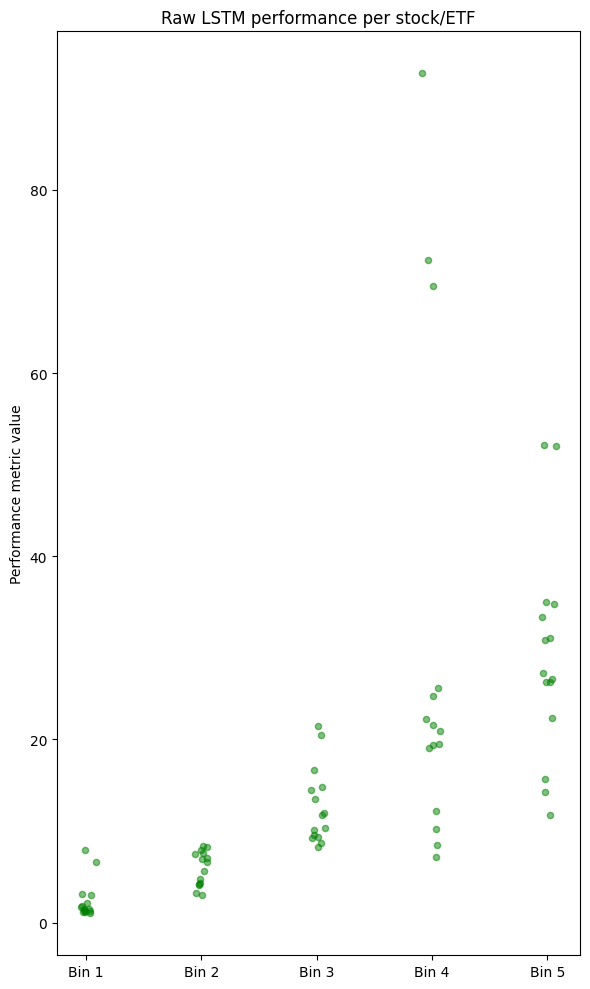
\includegraphics[width=0.5\textwidth]{images/results_LSTM.png}
  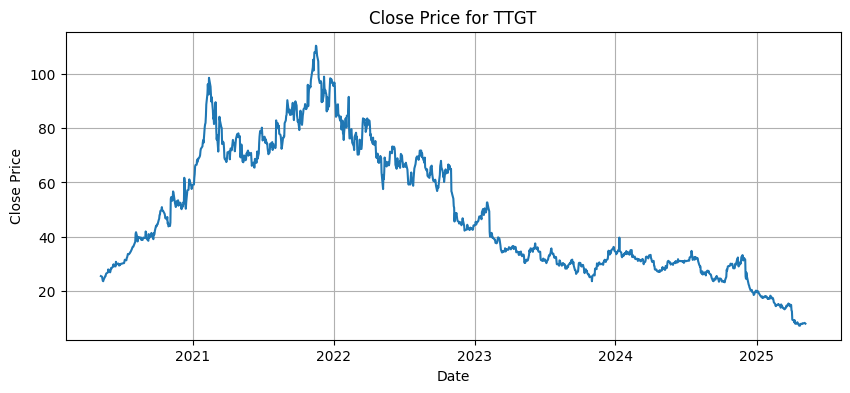
\includegraphics[width=0.5\textwidth]{images/outlier1.png}
  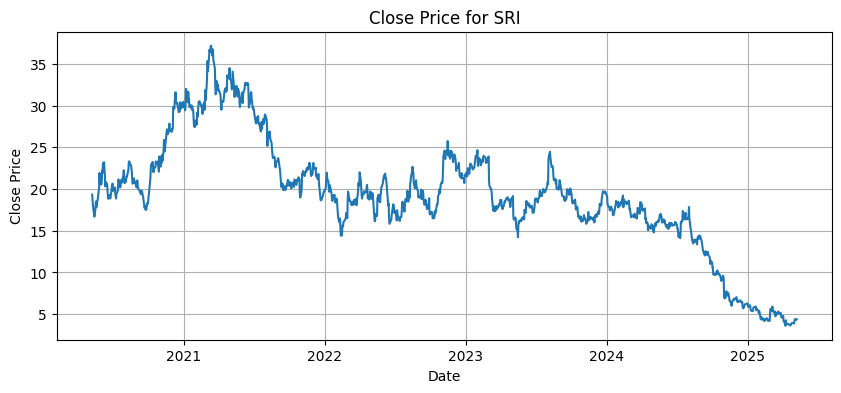
\includegraphics[width=0.5\textwidth]{images/outlier2.png}
  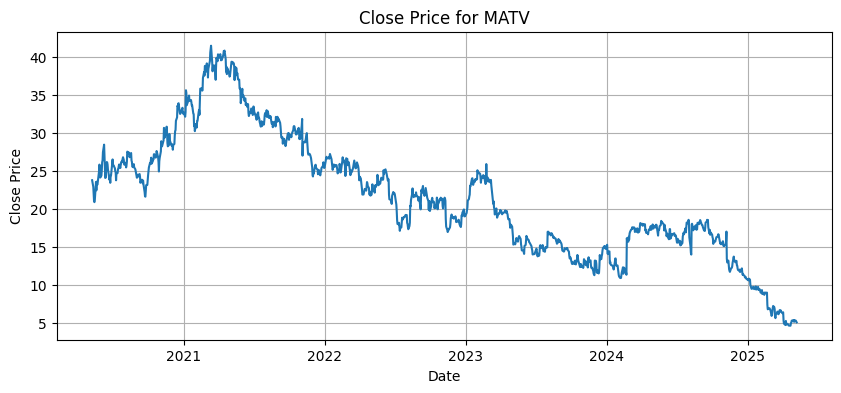
\includegraphics[width=0.5\textwidth]{images/outlier3.png}
  \caption{top: LSTM mape of single assets. bottom: 3/5 outliers }
  \label{fig:wrapped}
\end{wrapfigure}
		\subsubsection*{LSTM}
	In figure 6.1(top) we see the performance of forecasts for every single asset made by the LSTM model. The error which the performance is measured with here is the mape so that we can compare stocks across different scale. It is clearly visible that the average predictive performance is worse for assets of higher volatility. That makes absolute sense since noisier courses are harder to predict. We see some heavy outliers in bin 4 and bin 5. \\
	
	

		In figure 6.1(bottom) and 6.2 we look at the courses of these 5 assets and interestingly enough they all look very similar. It seems as if they all experience an uptrend throughout roughly the first quarter of the course and then a consistent downtrend. Another similarity is that it seems they are more volatile throughout the first half of the course and less volatile throughout the second half. These patterns might be especially hard for the model to learn because it first learns a highly volatile slight uptrend and then has to predict a rather smooth downtrend. If we take into consideration that we split the training data in a way where roughly the first 80\% of the course is training and only the last 10\% is test data, then this makes even more sense. Future research could focus on differentiating on this by evaluating average stocks against stocks with the described behavior. Another similarity seems to lie in the concrete price which the assets reach at the end of the captured time. All the courses seem to end below 10, some below 5. We know that the mape can explode for very low absolute values. We can not say for sure whether 10 would be small enough to cause trouble and lead to such heavy outliers. It could also be the case that this has nothing to do with the scale of these assets but that the model is just not performing as good as with the other assets. 
		
\begin{wrapfigure}{r}{0.5\textwidth}
  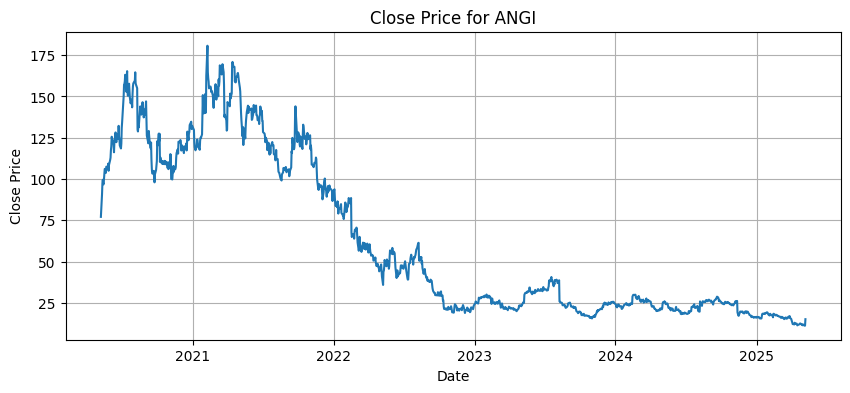
\includegraphics[width=0.5\textwidth]{images/outlier4.png}
  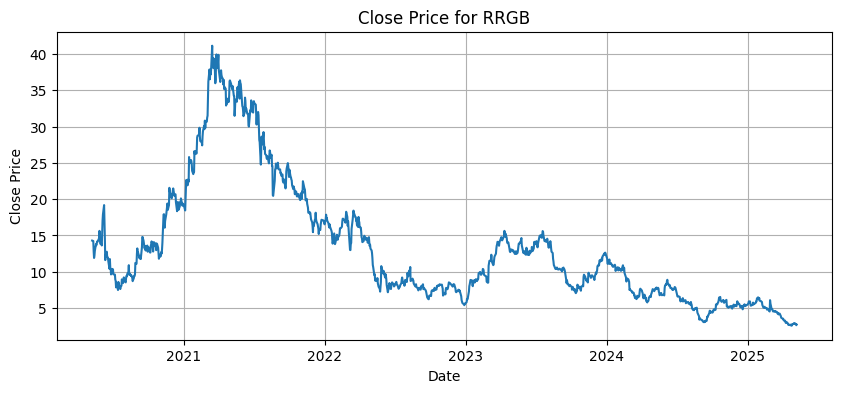
\includegraphics[width=0.5\textwidth]{images/outlier5.png}
  \caption{2/5 outliers}
  \label{fig:wrapped}
\end{wrapfigure}

Future research could focus on investigating this question by maybe predicting returns or log returns instead of raw prices. That would eliminate the problem of scale. Beyond that predicting returns and log returns in general has been observed to be good as forecasting target. In order to investigate these two questions we will conduct a little experiment. For that we modify our preprocessing pipeline to add the simple and logarithmic return of the close price. Once we have that we train the CNN and the XGBoost model again to evaluate them with better target engineering. We will include the results in the next sections when we look at the results for those two models. If we zoom out a bit and look at the mape averaged per bin, we get these results:\\\\
\begin{tabular}{|c|c|}
  \hline
  \textbf{Bin} & \textbf{Mean MAPE (\%)} \\
  \hline
  1 & 2.42 \\
  2 & 5.97 \\
  3 & 12.72 \\
  4 & 29.72 \\
  5 & 29.30 \\
  \hline
\end{tabular}\\

We can clearly confirm our statement from the beginning that the relative error correlates with the volatility. Besides that we want to understand how good our results are. A mape of 2.4 for bin 1 means that a prediction is on average off by 2.4\%. In order to say whether 2.4\% is good or bad we need to consider the volatility of the assets. \\\\

For that we pick two stocks out of bin 1 that have an approximate mape of 2.4, one has 3.1 and the other one has 2.1. We extract the ticker symbols and the volatility that we calculated in our stock selection pipeline and we see that their volatility is 0.24\% and 0.25\%. If the average forecast is off 2.1\% and one average period to period movement is 0.24\% then our forecast is not very useful. To be clear, an average error of 2.1\% at a volatility of 0.24\% is worse than just predicting the current days close price as tomorrows price. It underlines again how important a clear task formulation, good preprocessing and through thought model design is. 

\newpage
		\subsubsection*{CNN}
\begin{wrapfigure}{r}{0.5\textwidth}
  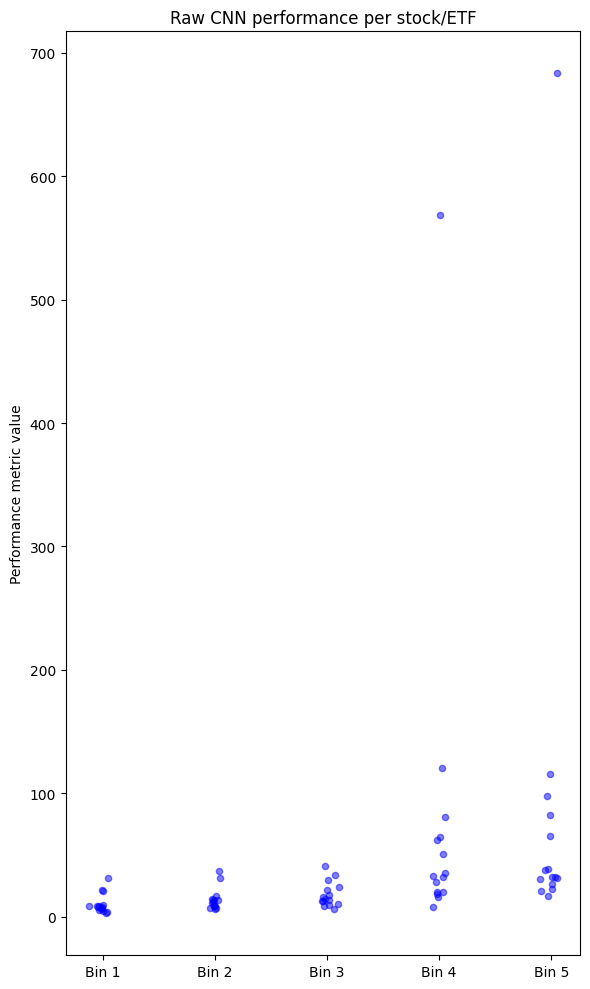
\includegraphics[width=0.5\textwidth]{images/results_CNN.png}
  \caption{CNN mape of single assets}
  \label{fig:wrapped}
\end{wrapfigure}

	
	Let’s now take a look at the CNN data. We first look at the performance based on predicting raw prices. We identify that the scale of this chart is much bigger. We see again two very heavy outliers at the top and also the correlation between the volatility and the mape seems to occur for the CNN model. The average volatility per bin for the CNN model is:
	\begin{tabular}{|c|c|}
  \hline
  \textbf{Bin} & \textbf{Mean MAPE (\%)} \\
  \hline
  1 & 10.32 \\
  2 & 13.98 \\
  3 & 18.21 \\
  4 & 77.21 \\
  5 & 88.99 \\
  \hline
\end{tabular}\\\\

	
	We can confirm the correlation between the relative error and volatility. The CNN model is worse than the LSTM model in terms of predictive accuracy. We can especially notice an immense increase in the error for bin 4 and 5. An mape of up to 88 is very much and possibly a consequence of predicting raw prices. \\
	
	When we zoom in on the predictive performance of the CNN when trained on the 5 stocks that led to outliers for the LSTM model, then we can see that it again has very bad performance for those. Two interesting things is that the outliers are not the same throughout. For example the CNN has a very high error for stock 1 and 2 from bin 5 while the performance of the LSTM model on this stocks is not very remarkable. This might be due to different strengths in the models regarding different data and could be further investigated by gathering more assets for which this unsymmetrical performance is occurring and then comparing these stocks against each other. 
	

		\subsubsection*{XGBoost}



When we look at the performance of the XGBoost model we again see a clear correlation between mape and volatility. We again see some outliers. When we look at the number it is interesting enough that the outliers we investigated for the LSTM model again are outliers for the XGBoost model. 

\begin{wrapfigure}{r}{0.5\textwidth}
  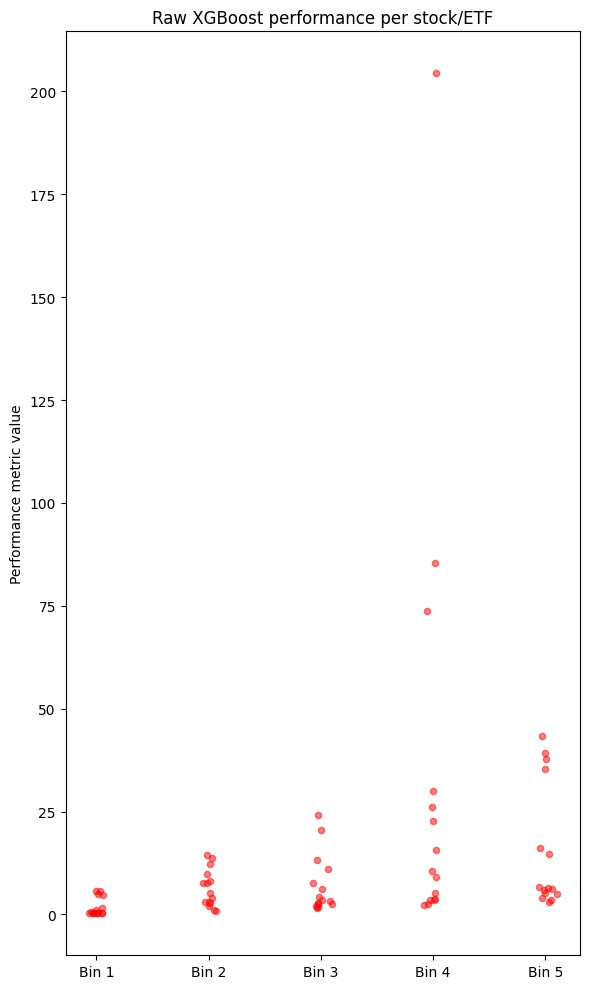
\includegraphics[width=0.5\textwidth]{images/results_XGBoost.png}
  \caption{XGBoost mape of single assets}
  \label{fig:wrapped}
\end{wrapfigure}


If all of the three models struggle to predict these assets accurately then it might be true that they have characteristics to them that make it much harder for the models to make precise forecasts. Let’s as well look at the forecasting performance averaged per bin:\\\\
	\begin{tabular}{|c|c|}
  \hline
  \textbf{Bin} & \textbf{Mean MAPE (\%)} \\
  \hline
  1 & 1.78 \\
  2 & 6.40 \\
  3 & 7.14 \\
  4 & 33.25 \\
  5 & 15.52 \\
  \hline
\end{tabular}\\\\
The XGBoost model seems to be dealing well with this task. Again it underperforms a simple baseline comparison as for example just predicting the current days close price as tomorrows. \\
We also notice that bin 5 has a much smaller mape than bin 4. If we look at the performance per stock, we see that is mostly due to a few very heavy outliers. Since we have not understood what causes this much worse performance for these certain stocks we can’t just leave them out. \\

		\subsubsection*{Comparison}



In figure 6.5(top) the performance of all three models is drawn in one graph. We can very clearly see the correlation between mape and volatility. It seems as the mape is increasing at the lowest rate with the volatility for the XGBoost model. So, the XGBoost model seems to be the best among our candidates to deal with high volatility data. To get a more precise comparison across the models we plot the averaged performance for all models bin wise. We see this bin wise performance in figure 6.5(bottom) First we notice that all courses have a similar shape. All have a slight increase in the mape over the first 3 bins and then suddenly the error increases by a lot for bin 4 and is about the same for bin 5 depending on the model. We see that the CNN model clearly performs worst among our candidates. The XGBoost and LSTM model seem to be very even in terms of their predictive accuracy. Remarkable is a sudden decrease in error of the XGBoost model for bin 5. That definitely is an interesting behavior and it underlines that the models have different strengths and weaknesses depending on the nature of data. As mentioned in our research question, in this thesis we aimed for understanding at which volatility the models perform best. Saying that the models perform best for a lower volatility seems to be the logical conclusion but if we want to precisely answer that question we would need to put the predictive performance into relation with the volatility.


\begin{wrapfigure}{r}{0.5\textwidth}
  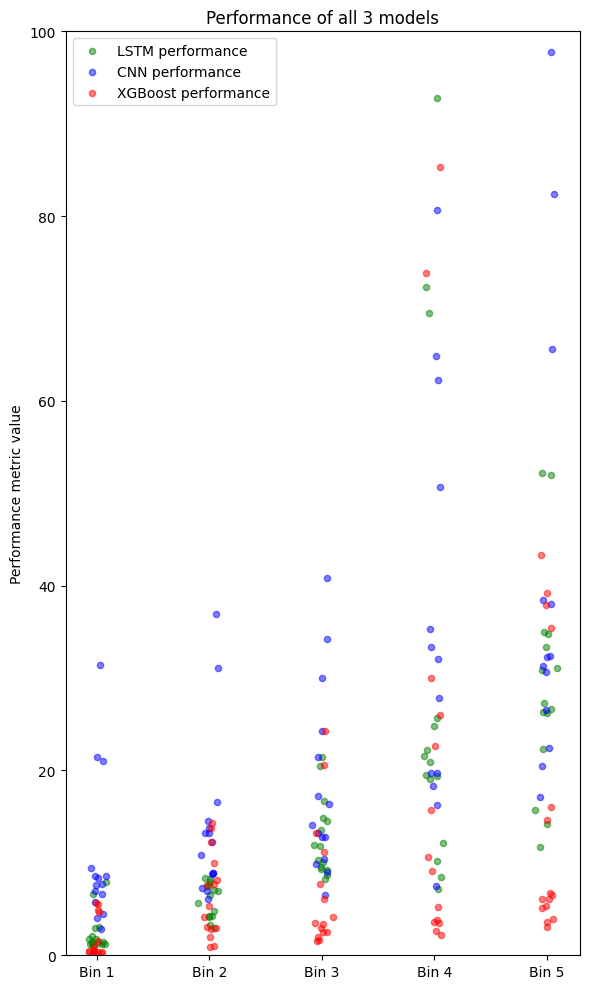
\includegraphics[width=0.5\textwidth]{images/results_combined.png}
  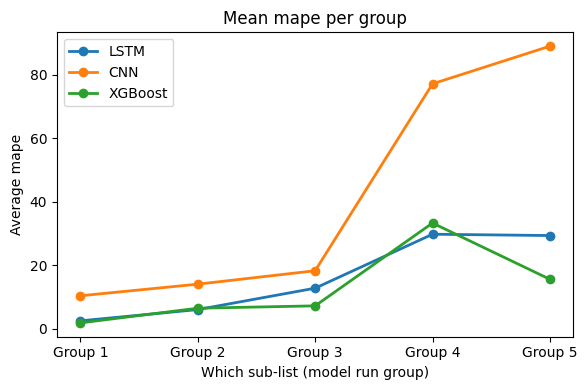
\includegraphics[width=0.5\textwidth]{images/results_averaged.png}
  \caption{top: combined mape of single assets. bottom: combined mape, averaged bin wise}
  \label{fig:wrapped}
\end{wrapfigure}

In other words, a model that is evaluated on two different stocks and has a similar predictive accuracy for both stocks performs better on the stock that has a higher volatility, since historical data with higher volatility is generally speaking more difficult to predict. To do so we simply divide the average mape for each bin by the volatility of that bin. In figure 6.6 the result of this transformation is drawn. Again the general shapes of all three models are similar. That indicates that characteristics in the data outweigh characteristics of the models. In fact the direction in which the mape moves between bins is for every pair of adjacent bins the same except for the difference of bin 2 and bin 3 where the mape of the LSTM increases slightly and the mape of CNN and XGBoost decreases. That shows beautifully how similar relative performance is between the models. Considering the execution times we can say that the XGBoost model clearly is the best performing model in this experiment. It has the shortest training duration among the three models in this experiment with 59 minutes. The LSTM model took about 32 times as long with about 1887 minutes. That is a relevant difference and definitely to be considered as part of the overall performance. The CNN model is in the middle field in terms of execution times with about 280 minutes but is clearly the worst in predictive accuracy which makes it a bad trade-off. The clear outperformer in this experiment is the XGBoost model. With the best average performance it is only challenged by the LSTM that has on average slightly less accurate predictions. If we also consider the fact that the XGBoost model had by far the shortest execution time with only one hour which is 32 times faster than the LSTM model, then it is clear that it is the preferred choice for similar tasks. The LSTM model had also a strong but not as good performance compared to the XGBoost model. The CNN model is far worse than both in forecasting accuracy. If we look at the execution time than we are left to say that the CNN model is much quicker compared to the LSTM model but performs much worse. A concrete trade-off point is hard to define here. For that we would need to precisely investigate how much more accurate the CNN model would make forecasts when trained and tuned for a longer time. The same applies to the LSTM model. How much worse would it be if only trained and tuned as long as the CNN model took? Would it still be better than the CNN model? This seems to be a rather complicated question and is not part of this thesis but could be subject of further research. 









\begin{figure}[htbp]
  \centering
  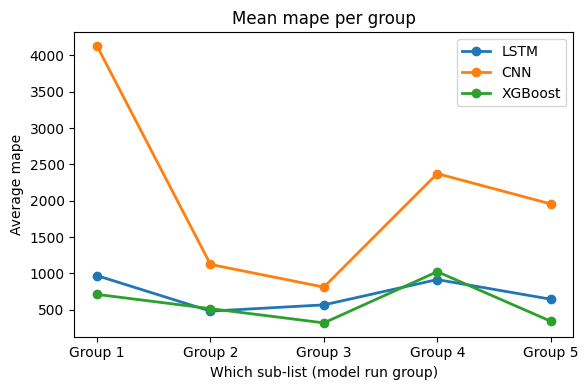
\includegraphics[width=0.5\textwidth]{images/averages_rescaled.png}
  \caption{bin wise average performance scaled with volatility}
  \label{fig:fullwidth}
\end{figure}



\subsection*{Future research}

In this thesis we showed the importance of qualitative preprocessing, accurate problem framing and model design. We showed how big the difference in predictive performance can be between a well selected, well-tuned model that is trained on clean preprocessed data and a model which seems to not be very suitable for such a task under these circumstances. There are many ways to get more insights in Future research could focus on further optimizing these tasks. This would be possible by tuning more hyperparameters for the models. For the XGBoost model this could for example be to also tune the size of lag values for each feature. In general the ranges from which the optuna study suggests values could be extended. 


\printbibliography





\newpage



\vspace*{\fill}         % push down to vertical center

{\fontsize{20}{23}\selectfont\textbf{Erklärung}}\\\\

Ich versichere, dass ich die vorliegende Arbeit selbstständig und nur unter Verwendung der
angegebenen Quellen und Hilfsmittel angefertigt habe, insbesondere sind wörtliche oder
sinngemäße Zitate als solche gekennzeichnet. Mir ist bekannt, dass Zuwiderhandlung auch
nachträglich zur Aberkennung des Abschlusses führen kann.
Ich versichere, dass das elektronische Exemplar mit den gedruckten Exemplaren übereinstimmt.\\\\

Ort:\\\\\\

Datum:\\\\\\

Unterschrift:\\\\\\\\\\

{\fontsize{20}{23}\selectfont\textbf{Declaration}}\\\\


I declare that I wrote this Thesis independently and only with usage of the specified aids and sources. Especially quotes are markes as such. I am aware that violation of that rule may lead to a revocation of my degree. I ensure that the electronic version is identical to the printed books.\\\\

Place:\\\\\\

Date:\\\\\\

Signature:
\vspace*{\fill}         % push the rest of the page down















\end{document}